\section{Anexo A. Bootstrap de todos los parámetros, descriptivas y efectos}\label{anx:A}

\setcounter{table}{0}\setcounter{figure}{0}\renewcommand{\thetable}{A-\arabic{table}}\renewcommand{\thefigure}{A-\arabic{figure}}

La tabla \ref{tab:A1} contiene los 128 estimandos de S1 de las familias parámetros (4), efectos (13) y descriptivas (111), con $B = 10.000$ remuestras cada uno (flujo \texttt{bootstrap\_parametros}). Para los estimandos globales se remuestrean filas completas; para diferencias y tasas por grupo, dentro de cada grupo. El IC clásico es el publicado en S1 (Wilson, $t$ o Welch) y solo existe para los parámetros y algunos efectos. Las notas (a)--(c) registran los casos en que el BCa no se estima o en que el bootstrap no tiene cobertura poblacional. Fuente: \texttt{outputs/validacion\_completa/tablas/bootstrap\_intervalos.csv}.

{\tiny\setlength{\tabcolsep}{3pt}
\begin{longtable}{@{}l >{\raggedright\arraybackslash}p{2.3cm} >{\raggedright\arraybackslash}p{2.0cm} r r l l l c@{}}
\caption{Bootstrap de los 128 estimandos de S1 ($B = 10.000$, IC al 95\,\%).}\label{tab:A1}\\\toprule
ID & Estimando & Grupo & $n$ & S1 & IC clásico S1 & IC percentil & IC BCa & Nota\\\midrule\endfirsthead
\multicolumn{9}{@{}l}{\emph{Continuación de la tabla \ref{tab:A1}}}\\\toprule
ID & Estimando & Grupo & $n$ & S1 & IC clásico S1 & IC percentil & IC BCa & Nota\\\midrule\endhead
\bottomrule\endfoot
PAR-001 & Media, costo & global & 10.999 & 210,20 & [209,30; 211,10] & [209,29; 211,10] & [209,29; 211,10] & \\
PAR-002 & Media, llamadas & global & 10.999 & 4,0545 & [4,0331; 4,0758] & [4,0327; 4,0756] & [4,0331; 4,0761] & \\
PAR-003 & Media, peso & global & 10.999 & 3.634,0 & [3.603,5; 3.664,6] & [3.603,8; 3.664,3] & [3.603,0; 3.663,8] & \\
PAR-004 & Proporción, atraso & 1 & 10.999 & 0,5967 & [0,5875; 0,6058] & [0,5876; 0,6060] & [0,5877; 0,6061] & \\
EFE-001 & $d_{av}$, compras previas & atras. $-$ punt. & 6.563/4.436 & $-$0,1133 & --- & [$-$0,1515; $-$0,0749] & [$-$0,1509; $-$0,0743] & \\
EFE-002 & $d_{av}$, costo & atras. $-$ punt. & 6.563/4.436 & $-$0,1505 & --- & [$-$0,1882; $-$0,1121] & [$-$0,1886; $-$0,1125] & \\
EFE-003 & $d_{av}$, descuento & atras. $-$ punt. & 6.563/4.436 & 0,9600 & --- & [0,9361; 0,9847] & [0,9357; 0,9842] & \\
EFE-004 & $d_{av}$, llamadas & atras. $-$ punt. & 6.563/4.436 & $-$0,1367 & --- & [$-$0,1749; $-$0,0987] & [$-$0,1753; $-$0,0991] & \\
EFE-005 & $d_{av}$, peso & atras. $-$ punt. & 6.563/4.436 & $-$0,5689 & --- & [$-$0,6105; $-$0,5277] & [$-$0,6100; $-$0,5273] & \\
EFE-006 & Dif. de medias, costo & atras. $-$ punt. & 6.563/4.436 & $-$7,2095 & [$-$9,0336; $-$5,3853] & [$-$8,9980; $-$5,3746] & [$-$9,0217; $-$5,3987] & \\
EFE-007 & Dif. de medias, descuento & atras. $-$ punt. & 6.563/4.436 & 13,12 & [12,65; 13,59] & [12,65; 13,60] & [12,65; 13,60] & \\
EFE-008 & Dif. de medias, peso & atras. $-$ punt. & 6.563/4.436 & $-$896,03 & [$-$956,03; $-$836,03] & [$-$955,60; $-$836,68] & [$-$954,57; $-$835,92] & \\
EFE-009 & Dif. de proporciones, descuento & Descuento $>$ 10 - Descuento $\le$ 10 & 2.647/8.352 & 0,5311 & [0,5203; 0,5418] & [0,5205; 0,5417] & [0,5205; 0,5418] & \\
EFE-010 & Dif. de proporciones, importancia & Importancia=alta - Importancia en \{baja, media\} & 948/10.051 & 0,0581 & [0,0257; 0,0893] & [0,0265; 0,0891] & [0,0265; 0,0891] & \\
EFE-011 & Biserial de rangos, peso & atras. $-$ punt. & 6.563/4.436 & $-$0,3130 & --- & [$-$0,3348; $-$0,2911] & [$-$0,3355; $-$0,2921] & \\
EFE-012 & Riesgo relativo, descuento & Descuento $>$ 10 / Descuento $\le$ 10 & 2.647/8.352 & 2,1328 & --- & [2,0854; 2,1818] & [2,0854; 2,1824] & \\
EFE-013 & Riesgo relativo, importancia & Importancia=alta / Importancia en \{baja, media\} & 948/10.051 & 1,0982 & --- & [1,0445; 1,1514] & [1,0445; 1,1514] & \\
DES-001 & Asimetría, compras previas & global & 10.999 & 1,6819 & --- & [1,6189; 1,7413] & [1,6200; 1,7423] & \\
DES-002 & Asimetría, costo & global & 10.999 & $-$0,1571 & --- & [$-$0,1868; $-$0,1270] & [$-$0,1869; $-$0,1270] & \\
DES-003 & Asimetría, descuento & global & 10.999 & 1,7989 & --- & [1,7425; 1,8556] & [1,7423; 1,8555] & \\
DES-004 & Asimetría, llamadas & global & 10.999 & 0,3919 & --- & [0,3592; 0,4249] & [0,3601; 0,4256] & \\
DES-005 & Asimetría, peso & global & 10.999 & $-$0,2497 & --- & [$-$0,2812; $-$0,2194] & [$-$0,2809; $-$0,2192] & \\
DES-006 & Curtosis (exceso), compras previas & global & 10.999 & 4,0063 & --- & [3,7313; 4,2724] & [3,7392; 4,2790] & \\
DES-007 & Curtosis (exceso), costo & global & 10.999 & $-$0,9722 & --- & [$-$1,0044; $-$0,9392] & [$-$1,0040; $-$0,9386] & \\
DES-008 & Curtosis (exceso), descuento & global & 10.999 & 2,0006 & --- & [1,7666; 2,2442] & [1,7677; 2,2446] & \\
DES-009 & Curtosis (exceso), llamadas & global & 10.999 & $-$0,3090 & --- & [$-$0,3641; $-$0,2513] & [$-$0,3647; $-$0,2519] & \\
DES-010 & Curtosis (exceso), peso & global & 10.999 & $-$1,4477 & --- & [$-$1,4731; $-$1,4198] & [$-$1,4733; $-$1,4201] & \\
DES-011 & DE, compras previas & global & 10.999 & 1,5229 & --- & [1,4881; 1,5577] & [1,4879; 1,5575] & \\
DES-012 & DE, costo & atrasada & 6.563 & 48,05 & --- & [47,48; 48,62] & [47,49; 48,63] & \\
DES-013 & DE, costo & global & 10.999 & 48,06 & --- & [47,60; 48,52] & [47,61; 48,53] & \\
DES-014 & DE, costo & puntual & 4.436 & 47,76 & --- & [47,01; 48,49] & [47,02; 48,50] & \\
DES-015 & DE, descuento & atrasada & 6.563 & 19,11 & --- & [18,81; 19,40] & [18,82; 19,40] & \\
DES-016 & DE, descuento & global & 10.999 & 16,21 & --- & [15,91; 16,51] & [15,91; 16,51] & \\
DES-017 & DE, descuento & puntual & 4.436 & 2,8777 & --- & [2,8396; 2,9144] & [2,8397; 2,9145] & \\
DES-018 & DE, llamadas & global & 10.999 & 1,1415 & --- & [1,1276; 1,1554] & [1,1280; 1,1558] & \\
DES-019 & DE, peso & atrasada & 6.563 & 1.576,1 & --- & [1.561,0; 1.590,8] & [1.561,2; 1.591,1] & \\
DES-020 & DE, peso & global & 10.999 & 1.635,4 & --- & [1.623,9; 1.646,6] & [1.624,2; 1.646,9] & \\
DES-021 & DE, peso & puntual & 4.436 & 1.574,0 & --- & [1.546,5; 1.600,3] & [1.547,0; 1.600,7] & \\
DES-022 & IQR, compras previas & global & 10.999 & 1,0000 & --- & [1,0000; 1,0000] & --- & b\\
DES-023 & IQR, costo & global & 10.999 & 82,00 & --- & [80,00; 83,00] & [81,00; 84,00] & \\
DES-024 & IQR, descuento & global & 10.999 & 6,0000 & --- & [6,0000; 6,0000] & --- & b\\
DES-025 & IQR, llamadas & global & 10.999 & 2,0000 & --- & [2,0000; 2,0000] & --- & a\\
DES-026 & IQR, peso & global & 10.999 & 3.210,5 & --- & [3.176,0; 3.243,5] & [3.178,0; 3.245,0] & \\
DES-027 & Máximo, compras previas & global & 10.999 & 10,00 & --- & [10,00; 10,00] & --- & a,c\\
DES-028 & Máximo, costo & global & 10.999 & 310,00 & --- & [310,00; 310,00] & --- & a,c\\
DES-029 & Máximo, descuento & global & 10.999 & 65,00 & --- & [65,00; 65,00] & --- & a,c\\
DES-030 & Máximo, llamadas & global & 10.999 & 7,0000 & --- & [7,0000; 7,0000] & --- & a,c\\
DES-031 & Máximo, peso & global & 10.999 & 7.846,0 & --- & [7.588,0; 7.846,0] & [7.684,0; 7.846,0] & c\\
DES-032 & Media, compras previas & atrasada & 6.563 & 3,4981 & --- & [3,4618; 3,5350] & [3,4627; 3,5362] & \\
DES-033 & Media, compras previas & global & 10.999 & 3,5676 & --- & [3,5390; 3,5965] & [3,5390; 3,5966] & \\
DES-034 & Media, compras previas & puntual & 4.436 & 3,6704 & --- & [3,6249; 3,7155] & [3,6256; 3,7160] & \\
DES-035 & Media, costo & atrasada & 6.563 & 207,29 & --- & [206,15; 208,44] & [206,11; 208,42] & \\
DES-036 & Media, costo & puntual & 4.436 & 214,50 & --- & [213,11; 215,92] & [213,11; 215,92] & \\
DES-037 & Media, descuento & atrasada & 6.563 & 18,66 & --- & [18,21; 19,13] & [18,21; 19,13] & \\
DES-038 & Media, descuento & global & 10.999 & 13,37 & --- & [13,08; 13,68] & [13,08; 13,68] & \\
DES-039 & Media, descuento & puntual & 4.436 & 5,5460 & --- & [5,4615; 5,6298] & [5,4602; 5,6289] & \\
DES-040 & Media, llamadas & atrasada & 6.563 & 3,9915 & --- & [3,9645; 4,0186] & [3,9645; 4,0186] & \\
DES-041 & Media, llamadas & puntual & 4.436 & 4,1477 & --- & [4,1132; 4,1819] & [4,1134; 4,1822] & \\
DES-042 & Media, peso & atrasada & 6.563 & 3.272,6 & --- & [3.234,4; 3.311,0] & [3.234,8; 3.311,4] & \\
DES-043 & Media, peso & puntual & 4.436 & 4.168,7 & --- & [4.122,5; 4.215,3] & [4.121,8; 4.214,7] & \\
DES-044 & Mediana, compras previas & atrasada & 6.563 & 3,0000 & --- & [3,0000; 3,0000] & --- & a\\
DES-045 & Mediana, compras previas & global & 10.999 & 3,0000 & --- & [3,0000; 3,0000] & --- & a\\
DES-046 & Mediana, compras previas & puntual & 4.436 & 3,0000 & --- & [3,0000; 3,0000] & --- & a\\
DES-047 & Mediana, costo & atrasada & 6.563 & 209,00 & --- & [207,00; 211,00] & --- & b\\
DES-048 & Mediana, costo & global & 10.999 & 214,00 & --- & [212,00; 216,00] & --- & b\\
DES-049 & Mediana, costo & puntual & 4.436 & 222,00 & --- & [219,00; 223,00] & --- & b\\
DES-050 & Mediana, descuento & atrasada & 6.563 & 9,0000 & --- & [9,0000; 9,0000] & --- & b\\
DES-051 & Mediana, descuento & global & 10.999 & 7,0000 & --- & [7,0000; 7,0000] & --- & a\\
DES-052 & Mediana, descuento & puntual & 4.436 & 6,0000 & --- & [5,0000; 6,0000] & --- & b\\
DES-053 & Mediana, llamadas & atrasada & 6.563 & 4,0000 & --- & [4,0000; 4,0000] & --- & a\\
DES-054 & Mediana, llamadas & global & 10.999 & 4,0000 & --- & [4,0000; 4,0000] & --- & a\\
DES-055 & Mediana, llamadas & puntual & 4.436 & 4,0000 & --- & [4,0000; 4,0000] & --- & a\\
DES-056 & Mediana, peso & atrasada & 6.563 & 3.231,0 & --- & [3.128,0; 3.332,0] & --- & b\\
DES-057 & Mediana, peso & global & 10.999 & 4.149,0 & --- & [4.120,0; 4.183,0] & --- & b\\
DES-058 & Mediana, peso & puntual & 4.436 & 4.674,0 & --- & [4.638,0; 4.715,0] & [4.638,0; 4.714,5] & \\
DES-059 & Mínimo, compras previas & global & 10.999 & 2,0000 & --- & [2,0000; 2,0000] & --- & a,c\\
DES-060 & Mínimo, costo & global & 10.999 & 96,00 & --- & [96,00; 96,00] & --- & b,c\\
DES-061 & Mínimo, descuento & global & 10.999 & 1,0000 & --- & [1,0000; 1,0000] & --- & a,c\\
DES-062 & Mínimo, llamadas & global & 10.999 & 2,0000 & --- & [2,0000; 2,0000] & --- & a,c\\
DES-063 & Mínimo, peso & global & 10.999 & 1.001,0 & --- & [1.001,0; 1.002,0] & --- & b,c\\
DES-064 & Extremos IQR (\%), costo & global & 10.999 & 0 & --- & [0; 0] & --- & a\\
DES-065 & Extremos IQR (\%), llamadas & global & 10.999 & 0 & --- & [0; 0] & --- & a\\
DES-066 & Extremos IQR (\%), peso & global & 10.999 & 0 & --- & [0; 0] & --- & a\\
DES-067 & \% suma top 1\%, costo & global & 10.999 & 1,4485 & --- & [1,4418; 1,4549] & [1,4421; 1,4552] & \\
DES-068 & \% suma top 1\%, llamadas & global & 10.999 & 1,7110 & --- & [1,7021; 1,7202] & [1,7019; 1,7200] & \\
DES-069 & \% suma top 1\%, peso & global & 10.999 & 1,6538 & --- & [1,6332; 1,6770] & [1,6350; 1,6800] & \\
DES-070 & Proporción, bodega & A & 10.999 & 0,1667 & --- & [0,1598; 0,1737] & [0,1597; 0,1737] & \\
DES-071 & Proporción, bodega & B & 10.999 & 0,1667 & --- & [0,1598; 0,1736] & [0,1598; 0,1737] & \\
DES-072 & Proporción, bodega & C & 10.999 & 0,1667 & --- & [0,1597; 0,1738] & [0,1597; 0,1736] & \\
DES-073 & Proporción, bodega & D & 10.999 & 0,1667 & --- & [0,1597; 0,1737] & [0,1597; 0,1739] & \\
DES-074 & Proporción, bodega & F & 10.999 & 0,3333 & --- & [0,3242; 0,3421] & [0,3245; 0,3424] & \\
DES-075 & Proporción, calificación & 1 & 10.999 & 0,2032 & --- & [0,1957; 0,2108] & [0,1957; 0,2108] & \\
DES-076 & Proporción, calificación & 2 & 10.999 & 0,1968 & --- & [0,1895; 0,2043] & [0,1895; 0,2043] & \\
DES-077 & Proporción, calificación & 3 & 10.999 & 0,2036 & --- & [0,1961; 0,2111] & [0,1961; 0,2111] & \\
DES-078 & Proporción, calificación & 4 & 10.999 & 0,1990 & --- & [0,1916; 0,2065] & [0,1916; 0,2065] & \\
DES-079 & Proporción, calificación & 5 & 10.999 & 0,1974 & --- & [0,1899; 0,2047] & [0,1901; 0,2049] & \\
DES-080 & Proporción, atraso & 0 & 10.999 & 0,4033 & --- & [0,3940; 0,4124] & [0,3939; 0,4123] & \\
DES-081 & Proporción, género & F & 10.999 & 0,5041 & --- & [0,4947; 0,5135] & [0,4949; 0,5138] & \\
DES-082 & Proporción, género & M & 10.999 & 0,4959 & --- & [0,4865; 0,5053] & [0,4862; 0,5051] & \\
DES-083 & Proporción, importancia & high & 10.999 & 0,0862 & --- & [0,0809; 0,0915] & [0,0809; 0,0915] & \\
DES-084 & Proporción, importancia & low & 10.999 & 0,4816 & --- & [0,4720; 0,4908] & [0,4723; 0,4910] & \\
DES-085 & Proporción, importancia & medium & 10.999 & 0,4322 & --- & [0,4231; 0,4416] & [0,4229; 0,4415] & \\
DES-086 & Proporción, modalidad & Flight & 10.999 & 0,1616 & --- & [0,1547; 0,1684] & [0,1547; 0,1685] & \\
DES-087 & Proporción, modalidad & Road & 10.999 & 0,1600 & --- & [0,1531; 0,1669] & [0,1531; 0,1670] & \\
DES-088 & Proporción, modalidad & Ship & 10.999 & 0,6784 & --- & [0,6695; 0,6872] & [0,6695; 0,6871] & \\
DES-089 & Q1, compras previas & global & 10.999 & 3,0000 & --- & [3,0000; 3,0000] & --- & b\\
DES-090 & Q1, costo & global & 10.999 & 169,00 & --- & [168,00; 171,00] & [167,00; 170,00] & \\
DES-091 & Q1, descuento & global & 10.999 & 4,0000 & --- & [4,0000; 4,0000] & --- & a\\
DES-092 & Q1, llamadas & global & 10.999 & 3,0000 & --- & [3,0000; 3,0000] & --- & a\\
DES-093 & Q1, peso & global & 10.999 & 1.839,5 & --- & [1.817,0; 1.866,0] & [1.817,0; 1.866,0] & \\
DES-094 & Q3, compras previas & global & 10.999 & 4,0000 & --- & [4,0000; 4,0000] & --- & a\\
DES-095 & Q3, costo & global & 10.999 & 251,00 & --- & [250,00; 252,00] & --- & b\\
DES-096 & Q3, descuento & global & 10.999 & 10,00 & --- & [10,00; 10,00] & --- & b\\
DES-097 & Q3, llamadas & global & 10.999 & 5,0000 & --- & [5,0000; 5,0000] & --- & a\\
DES-098 & Q3, peso & global & 10.999 & 5.050,0 & --- & [5.017,0; 5.082,0] & [5.017,0; 5.081,5] & \\
DES-099 & Tasa de atraso, bodega & Bodega=A & 1.833 & 0,5865 & --- & [0,5641; 0,6083] & [0,5641; 0,6083] & \\
DES-100 & Tasa de atraso, bodega & Bodega=B & 1.833 & 0,6023 & --- & [0,5799; 0,6247] & [0,5794; 0,6241] & \\
DES-101 & Tasa de atraso, calificación & Calificación=1 & 2.235 & 0,5875 & --- & [0,5669; 0,6081] & [0,5673; 0,6085] & \\
DES-102 & Tasa de atraso, calificación & Calificación=5 & 2.171 & 0,6066 & --- & [0,5854; 0,6274] & [0,5854; 0,6274] & \\
DES-103 & Tasa de atraso, descuento & Descuento $\le$ 10 & 8.352 & 0,4689 & [0,4582; 0,4796] & [0,4583; 0,4795] & [0,4582; 0,4795] & \\
DES-104 & Tasa de atraso, descuento & Descuento $>$ 10 & 2.647 & 1,0000 & [0,9986; 1,0000] & [1,0000; 1,0000] & --- & a\\
DES-105 & Tasa de atraso, género & Género=Fem. & 5.545 & 0,5944 & --- & [0,5816; 0,6076] & [0,5814; 0,6074] & \\
DES-106 & Tasa de atraso, género & Género=Masc. & 5.454 & 0,5990 & --- & [0,5860; 0,6120] & [0,5860; 0,6118] & \\
DES-107 & Tasa de atraso, importancia & Importancia en \{baja, media\} & 10.051 & 0,5917 & --- & [0,5821; 0,6014] & [0,5821; 0,6014] & \\
DES-108 & Tasa de atraso, importancia & Importancia=alta & 948 & 0,6498 & --- & [0,6192; 0,6804] & [0,6192; 0,6804] & \\
DES-109 & Tasa de atraso, importancia & Importancia=media & 4.754 & 0,5905 & --- & [0,5766; 0,6045] & [0,5761; 0,6041] & \\
DES-110 & Tasa de atraso, modalidad & Modalidad=Avión & 1.777 & 0,6016 & --- & [0,5791; 0,6241] & [0,5779; 0,6235] & \\
DES-111 & Tasa de atraso, modalidad & Modalidad=Carretera & 1.760 & 0,5881 & --- & [0,5648; 0,6114] & [0,5648; 0,6114] & \\
\end{longtable}}
{\footnotesize (a) Réplicas constantes: distribución degenerada, BCa no estimable (por ejemplo, la tasa de atraso con descuento $> 10$, siempre 1). (b) \emph{Jackknife} sin variación: aceleración no estimable. (c) Extremo muestral: solo diagnóstico descriptivo, sin cobertura poblacional. Montos en USD, pesos en gramos, proporciones entre 0 y 1.\par}\medskip

Las figuras \ref{fig:A1}--\ref{fig:A11} muestran la distribución \emph{bootstrap} de cada estimando con sus intervalos (atlas completo).

\begin{figure}[H]\centering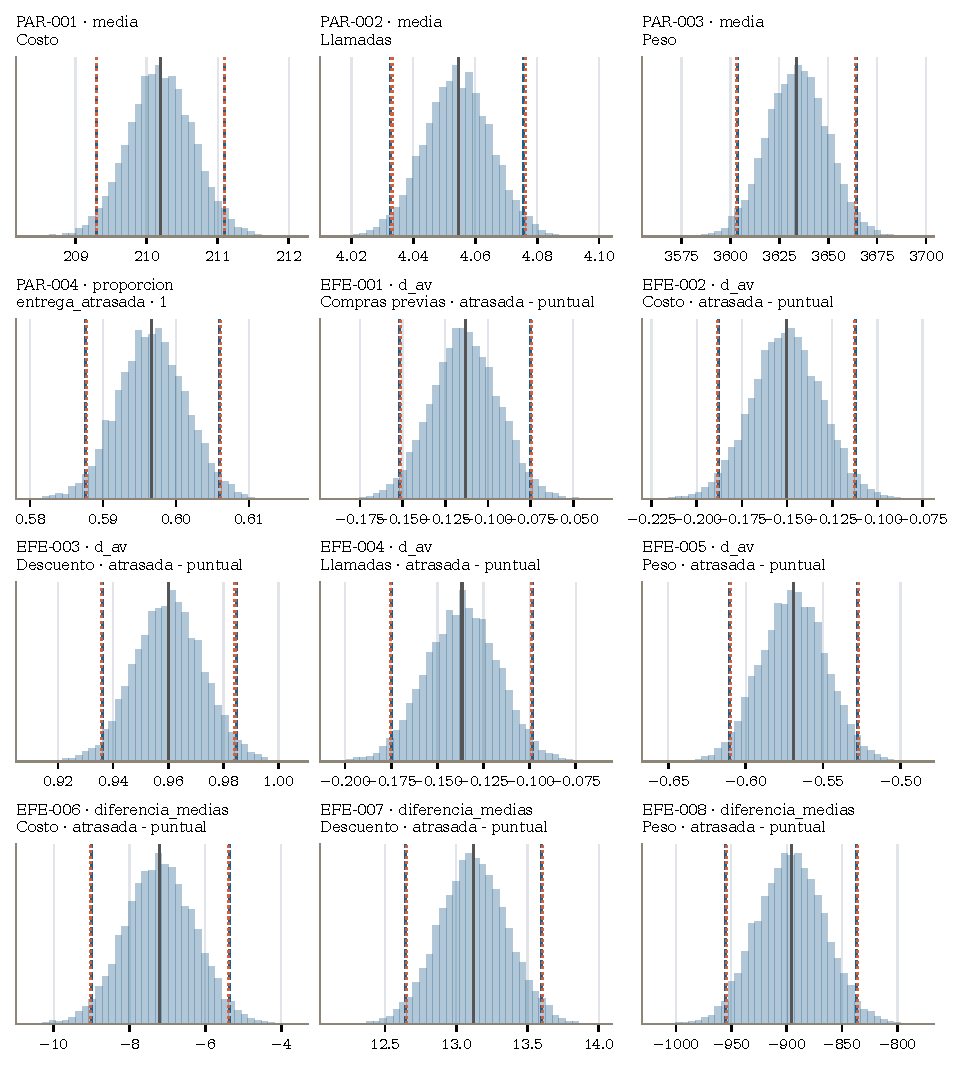
\includegraphics[width=\linewidth,height=0.40\textheight,keepaspectratio]{../../outputs/validacion_completa/figuras/fig_boot_A01_atlas.pdf}\caption{Atlas de distribuciones \emph{bootstrap}, parte 1 de 11.}\label{fig:A1}\end{figure}

\begin{figure}[H]\centering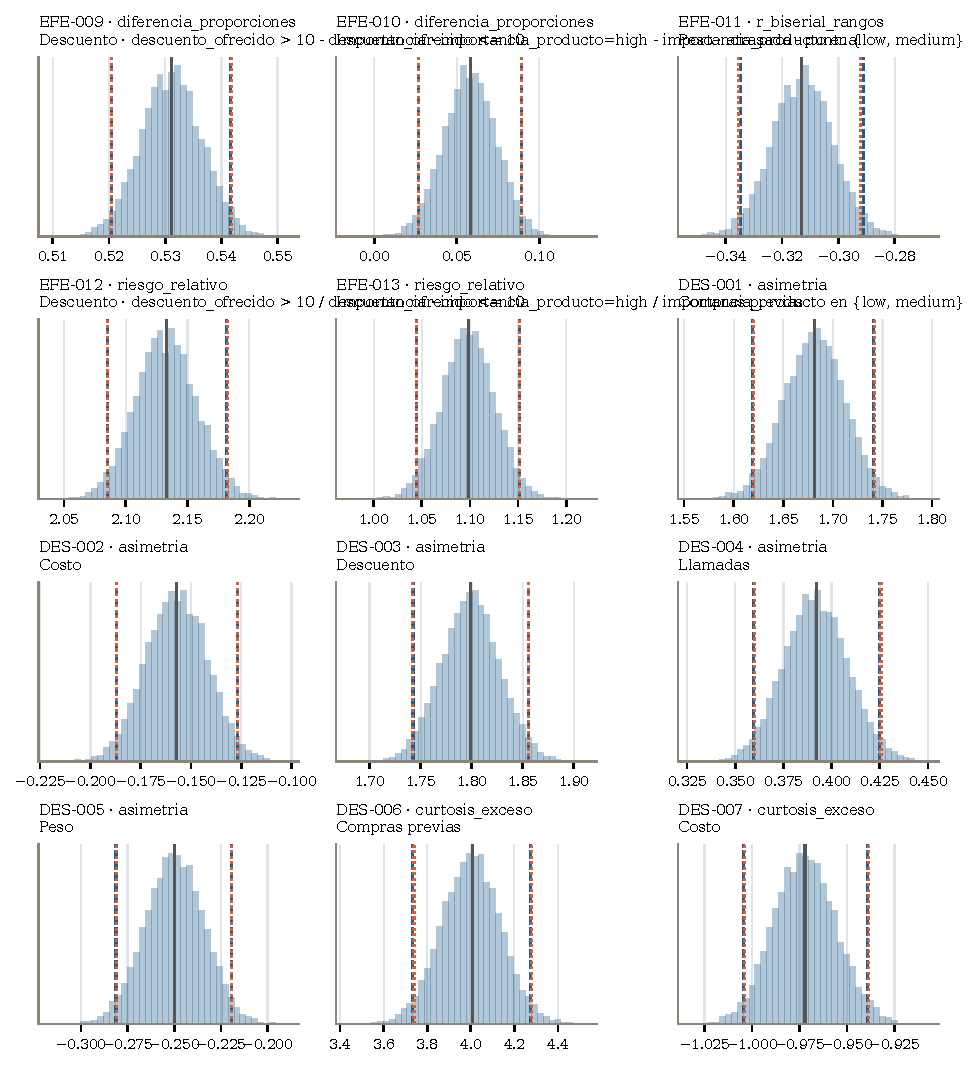
\includegraphics[width=\linewidth,height=0.40\textheight,keepaspectratio]{../../outputs/validacion_completa/figuras/fig_boot_A02_atlas.pdf}\caption{Atlas de distribuciones \emph{bootstrap}, parte 2 de 11.}\label{fig:A2}\end{figure}

\begin{figure}[H]\centering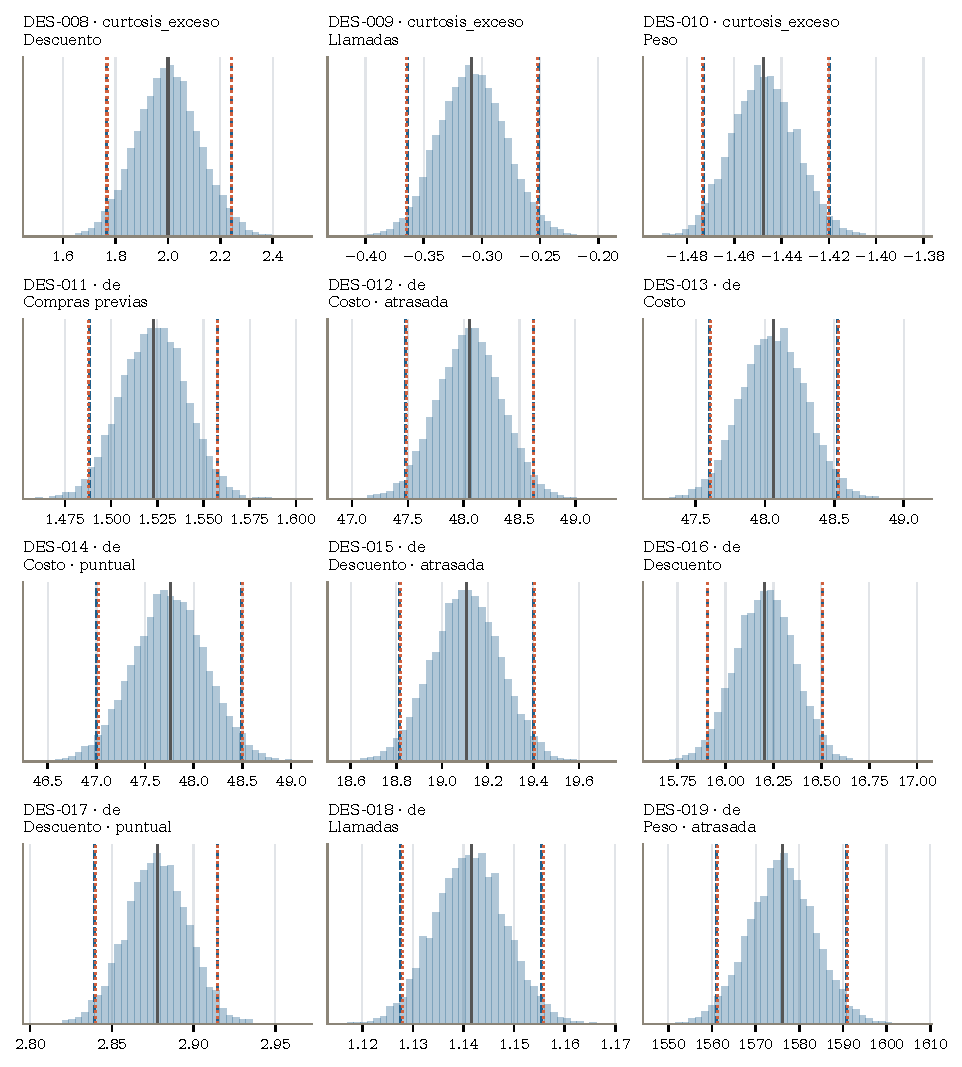
\includegraphics[width=\linewidth,height=0.40\textheight,keepaspectratio]{../../outputs/validacion_completa/figuras/fig_boot_A03_atlas.pdf}\caption{Atlas de distribuciones \emph{bootstrap}, parte 3 de 11.}\label{fig:A3}\end{figure}

\begin{figure}[H]\centering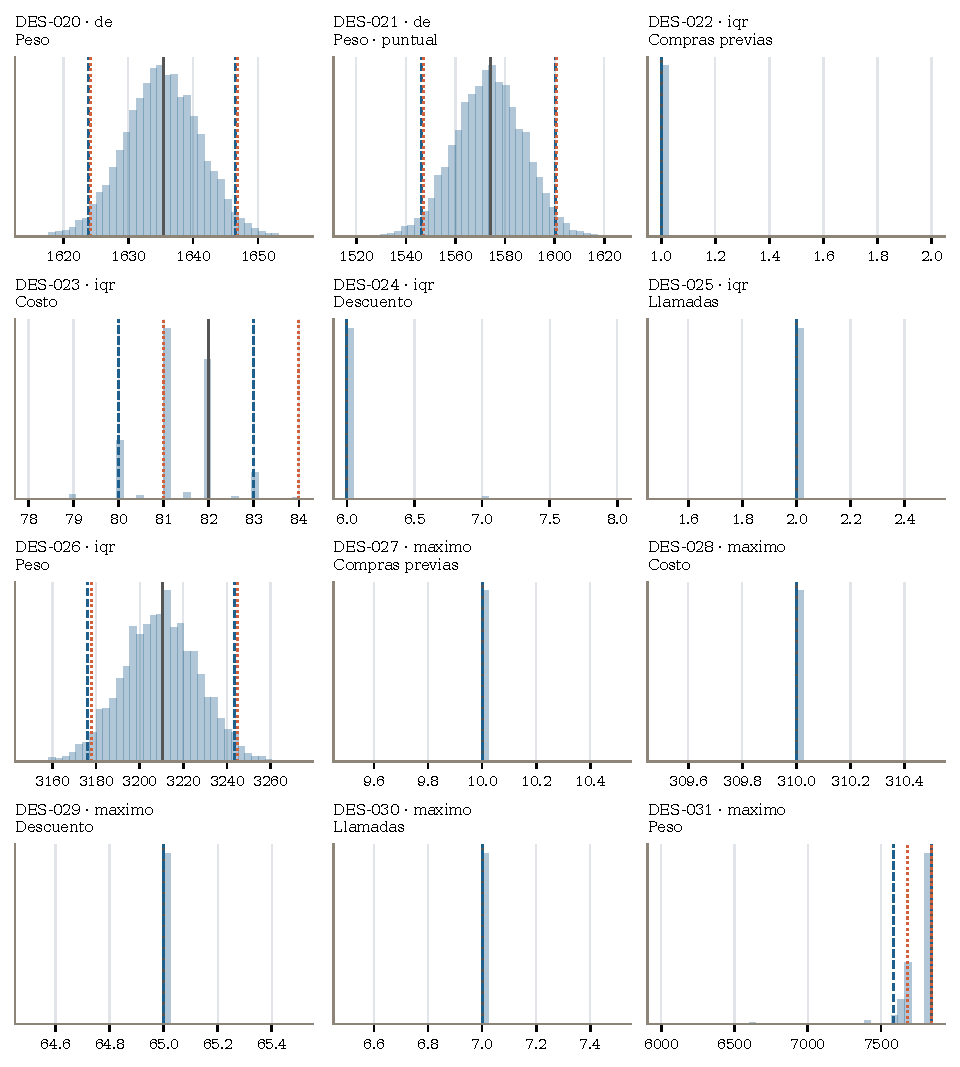
\includegraphics[width=\linewidth,height=0.40\textheight,keepaspectratio]{../../outputs/validacion_completa/figuras/fig_boot_A04_atlas.pdf}\caption{Atlas de distribuciones \emph{bootstrap}, parte 4 de 11.}\label{fig:A4}\end{figure}

\begin{figure}[H]\centering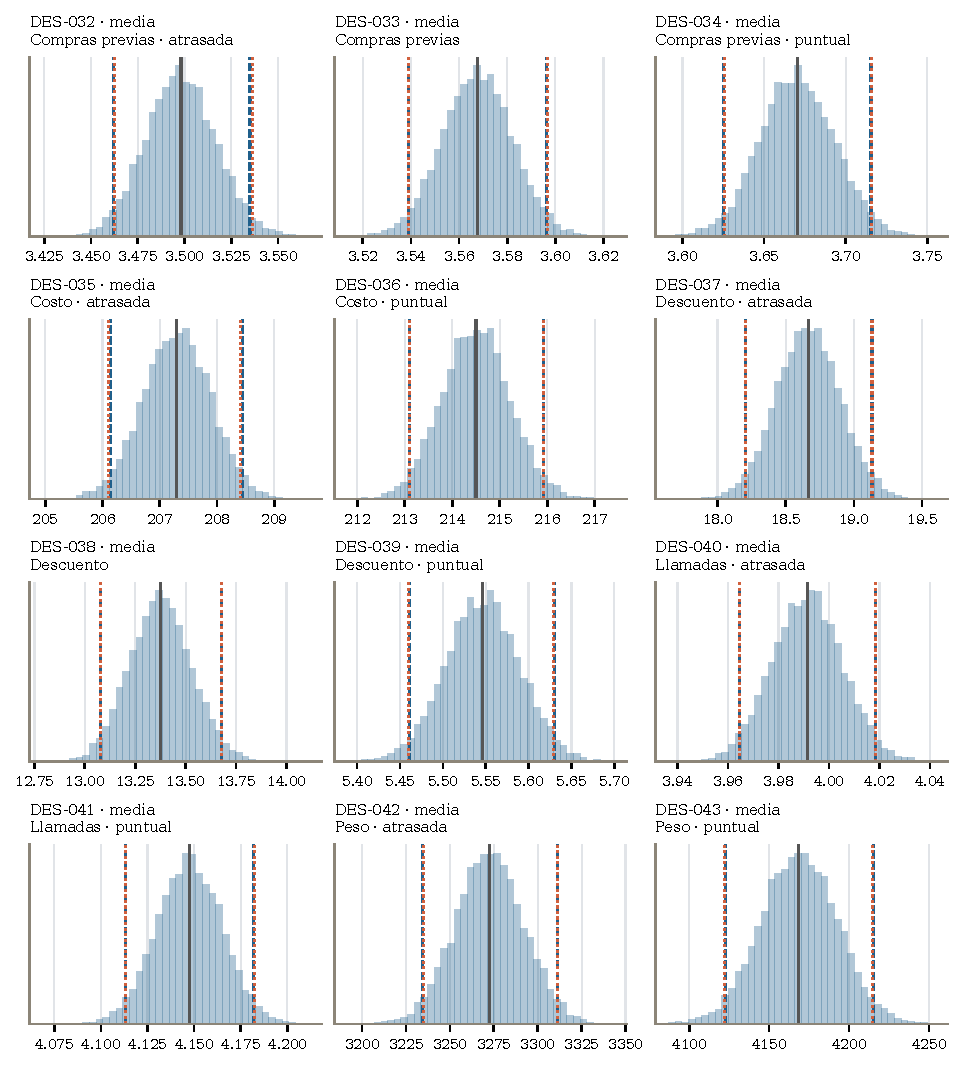
\includegraphics[width=\linewidth,height=0.40\textheight,keepaspectratio]{../../outputs/validacion_completa/figuras/fig_boot_A05_atlas.pdf}\caption{Atlas de distribuciones \emph{bootstrap}, parte 5 de 11.}\label{fig:A5}\end{figure}

\begin{figure}[H]\centering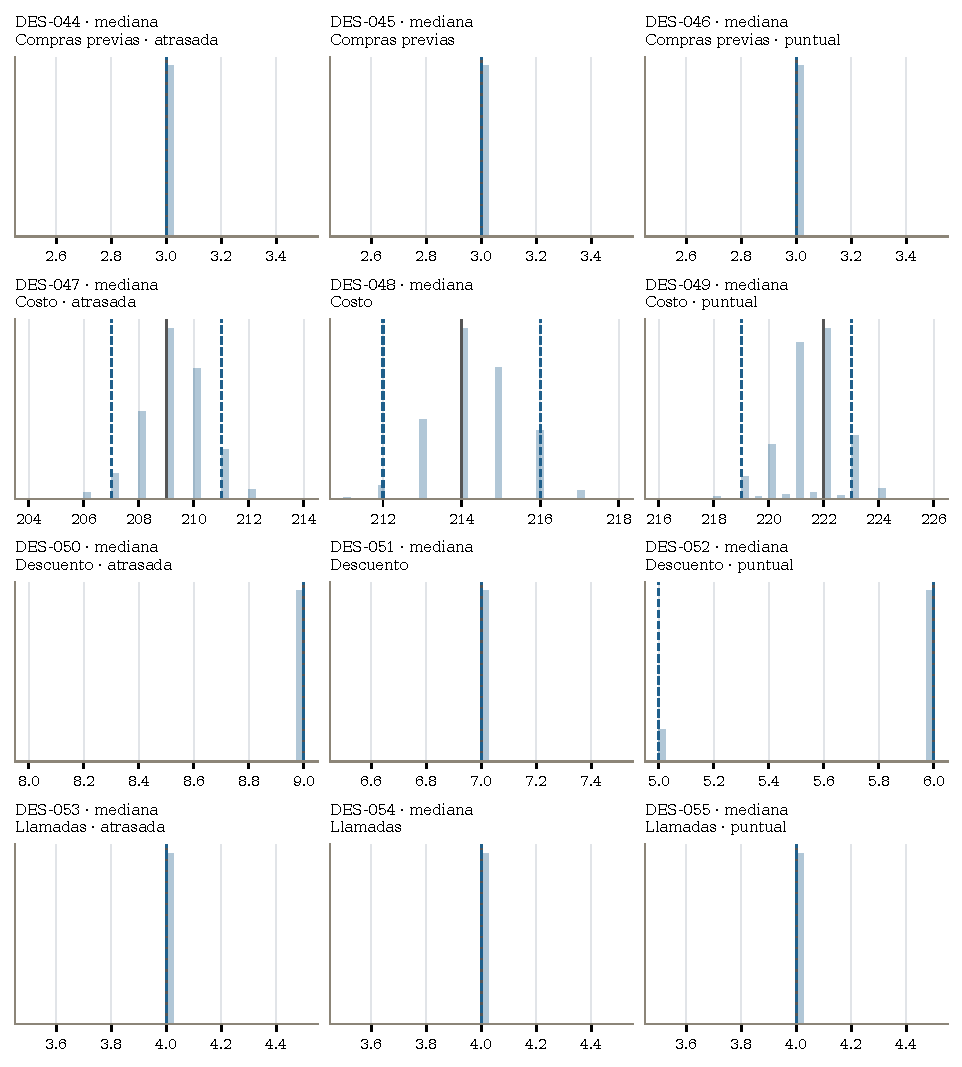
\includegraphics[width=\linewidth,height=0.40\textheight,keepaspectratio]{../../outputs/validacion_completa/figuras/fig_boot_A06_atlas.pdf}\caption{Atlas de distribuciones \emph{bootstrap}, parte 6 de 11.}\label{fig:A6}\end{figure}

\begin{figure}[H]\centering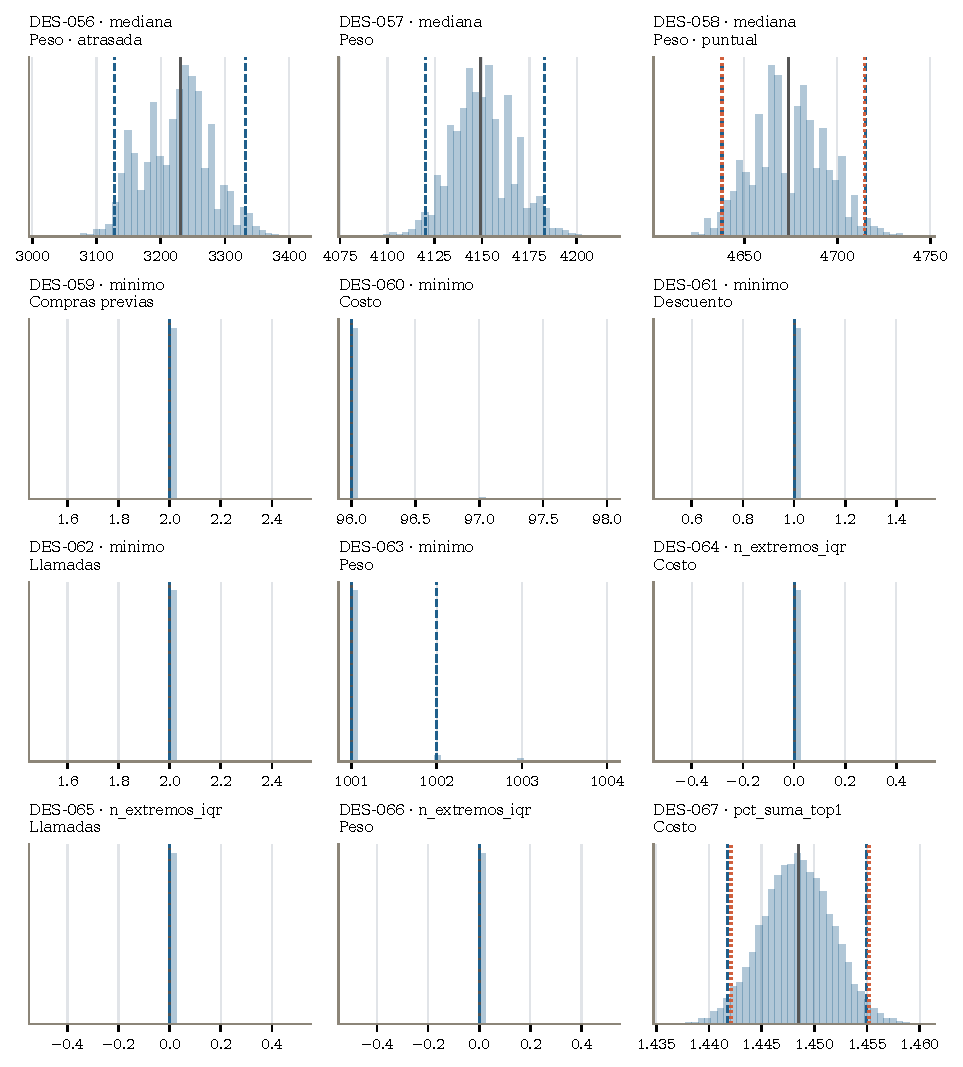
\includegraphics[width=\linewidth,height=0.40\textheight,keepaspectratio]{../../outputs/validacion_completa/figuras/fig_boot_A07_atlas.pdf}\caption{Atlas de distribuciones \emph{bootstrap}, parte 7 de 11.}\label{fig:A7}\end{figure}

\begin{figure}[H]\centering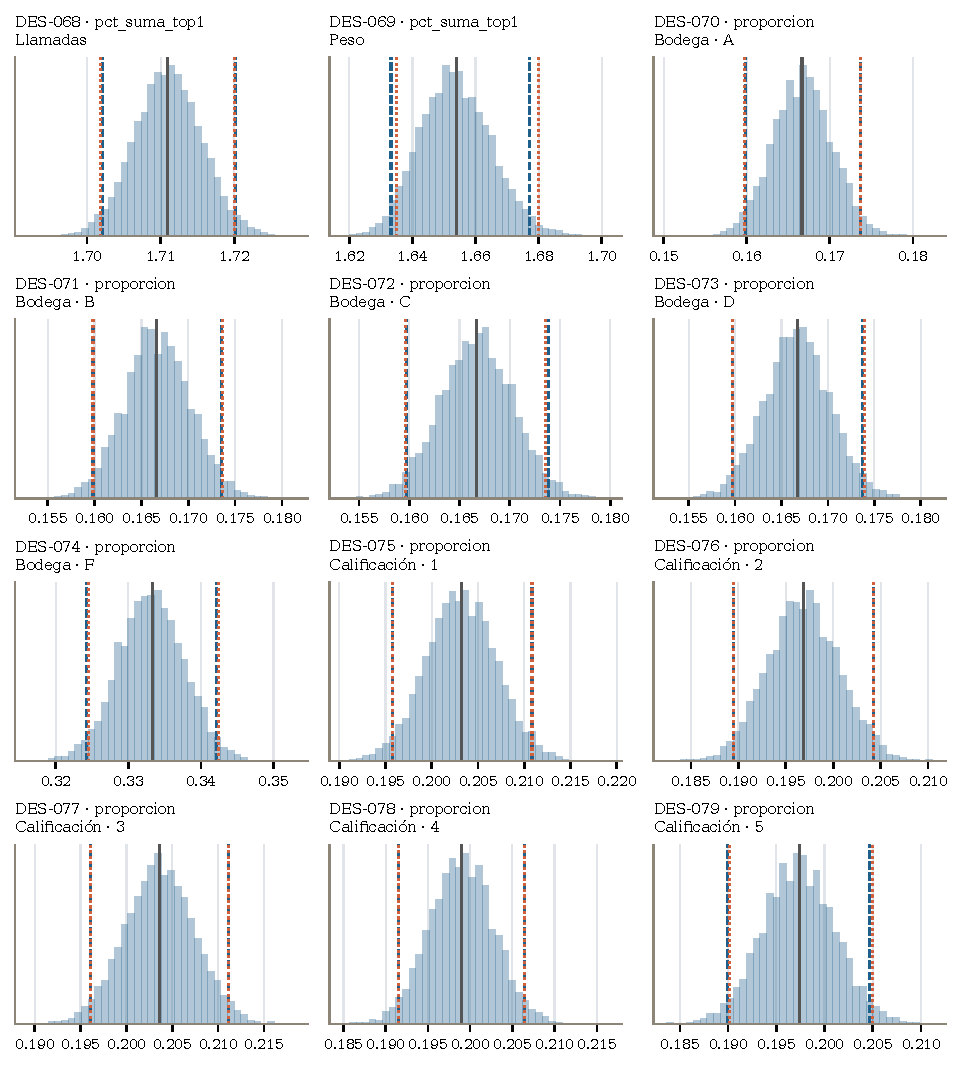
\includegraphics[width=\linewidth,height=0.40\textheight,keepaspectratio]{../../outputs/validacion_completa/figuras/fig_boot_A08_atlas.pdf}\caption{Atlas de distribuciones \emph{bootstrap}, parte 8 de 11.}\label{fig:A8}\end{figure}

\begin{figure}[H]\centering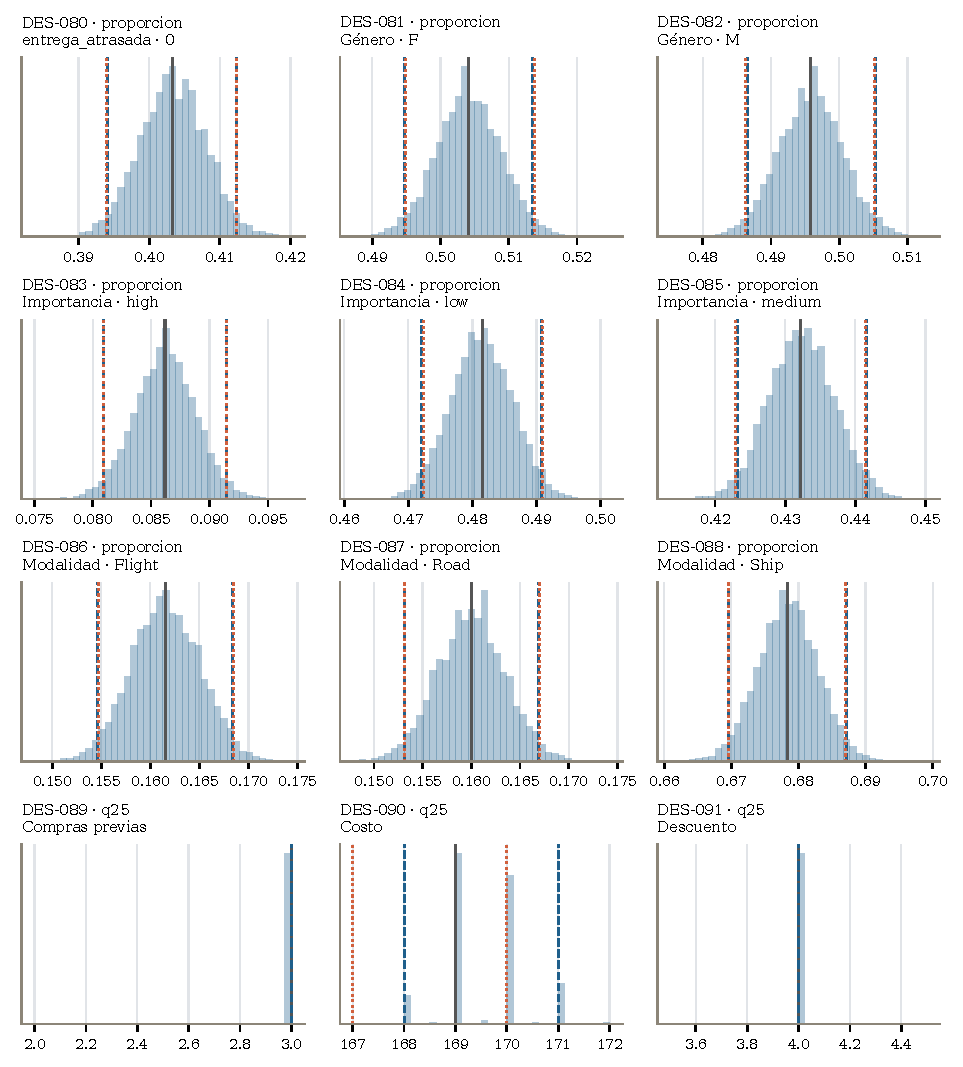
\includegraphics[width=\linewidth,height=0.40\textheight,keepaspectratio]{../../outputs/validacion_completa/figuras/fig_boot_A09_atlas.pdf}\caption{Atlas de distribuciones \emph{bootstrap}, parte 9 de 11.}\label{fig:A9}\end{figure}

\begin{figure}[H]\centering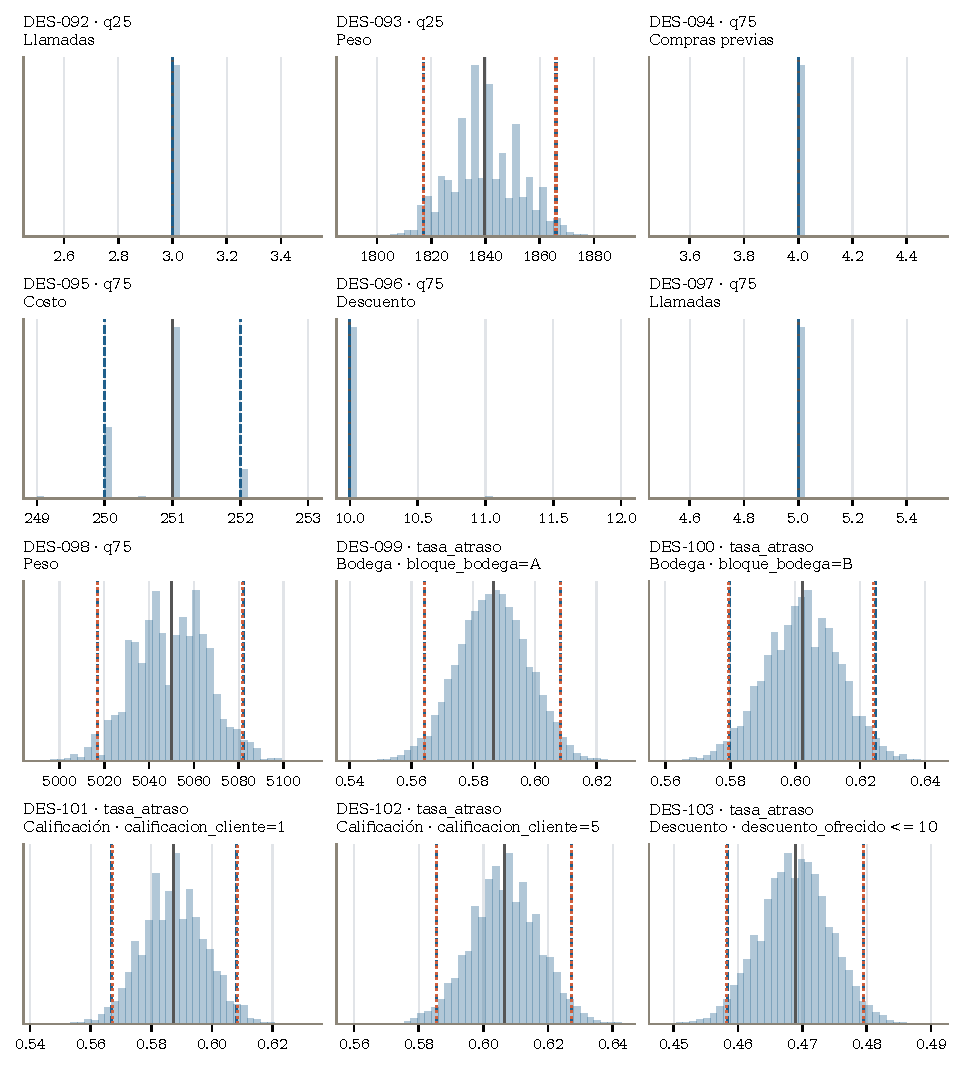
\includegraphics[width=\linewidth,height=0.40\textheight,keepaspectratio]{../../outputs/validacion_completa/figuras/fig_boot_A10_atlas.pdf}\caption{Atlas de distribuciones \emph{bootstrap}, parte 10 de 11.}\label{fig:A10}\end{figure}

\begin{figure}[H]\centering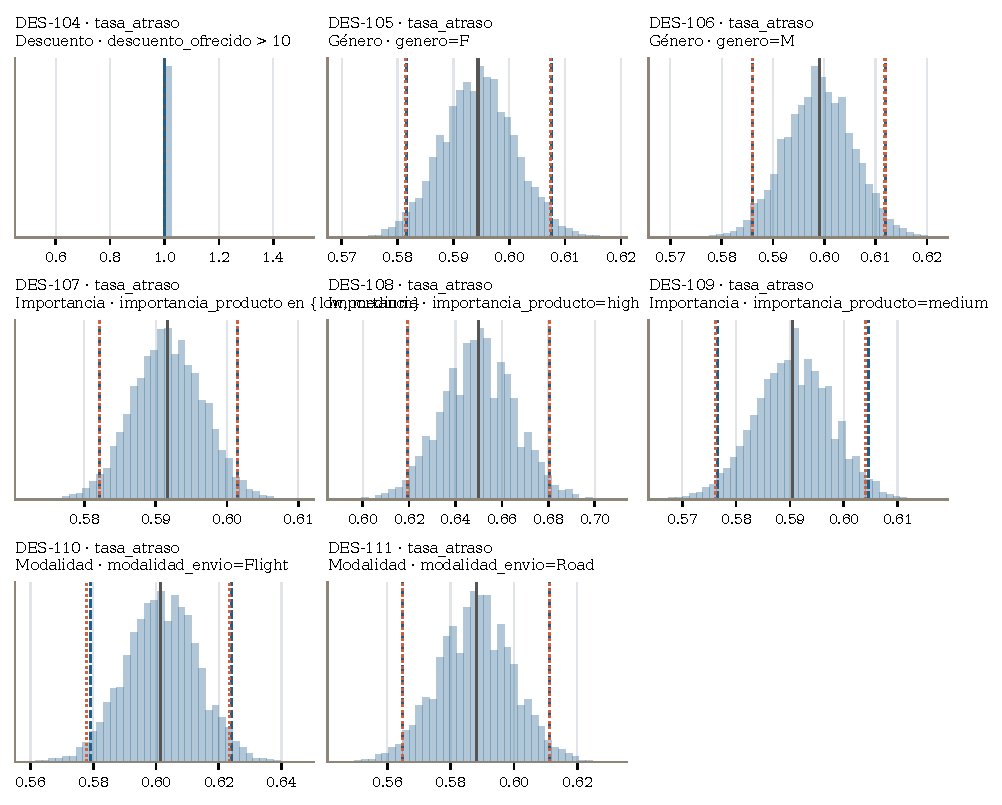
\includegraphics[width=\linewidth,height=0.40\textheight,keepaspectratio]{../../outputs/validacion_completa/figuras/fig_boot_A11_atlas.pdf}\caption{Atlas de distribuciones \emph{bootstrap}, parte 11 de 11.}\label{fig:A11}\end{figure}

\clearpage\section{Anexo B. Permutación de las siete pruebas de S1}\label{anx:B}

\setcounter{table}{0}\setcounter{figure}{0}\renewcommand{\thetable}{B-\arabic{table}}\renewcommand{\thefigure}{B-\arabic{figure}}

Cada prueba conserva la hipótesis, los grupos y el estadístico de S1, recalculado en cada una de las $B = 10.000$ permutaciones (flujo \texttt{permutaciones}). Se usa $p_{perm} = (1 + \text{excedencias})/(B + 1)$, con resolución $1/10.001$; cola superior para $\chi^2$, bilateral para $t$ y $z$, y distancia al centro $n_1 n_0/2$ para $U$. Holm se aplica a la familia de los siete $p$ de permutación y se compara con la familia Holm de S1. Fuente: \texttt{permutaciones\_todas.csv}.

{\scriptsize\setlength{\tabcolsep}{3pt}
\begin{longtable}{@{}l l l r r r r r r r c@{}}
\caption{Siete pruebas de S1: valor $p$ de permutación frente al paramétrico, crudo y con Holm.}\label{tab:B1}\\\toprule
ID & Variable & Estad. & Observado & Efecto & Exced. & $p_{perm}$ & Holm perm. & $p$ S1 & Holm S1 & Conc.\\\midrule\endfirsthead
\multicolumn{11}{@{}l}{\emph{Continuación de la tabla \ref{tab:B1}}}\\\toprule
ID & Variable & Estad. & Observado & Efecto & Exced. & $p_{perm}$ & Holm perm. & $p$ S1 & Holm S1 & Conc.\\\midrule\endhead
\bottomrule\endfoot
T01 & Modalidad & $\chi^2$ & 0,7434 & 0,0082 & 6.911 & 0,6911 & 0,6911 & 0,6895 & 0,6895 & Sí\\
T02 & Peso & $t$ Welch & $-$29,27 & $-$896,03 & 0 & $1{,}00\cdot 10^{-4}$ & $7{,}00\cdot 10^{-4}$ & $1{,}93\cdot 10^{-180}$ & $9{,}65\cdot 10^{-180}$ & Sí\\
T03 & Descuento & $t$ Welch & 54,70 & 13,12 & 0 & $1{,}00\cdot 10^{-4}$ & $7{,}00\cdot 10^{-4}$ & 0\textsuperscript{s} & 0\textsuperscript{s} & Sí\\
E1 & Peso (rangos) & $U$ & 10.000.332,5 & $-$0,3130 & 0 & $1{,}00\cdot 10^{-4}$ & $7{,}00\cdot 10^{-4}$ & $3{,}40\cdot 10^{-171}$ & $1{,}36\cdot 10^{-170}$ & Sí\\
E2 & Importancia alta & $z$ & 3,4863 & 0,0581 & 7 & $8{,}00\cdot 10^{-4}$ & 0,0016 & $4{,}90\cdot 10^{-4}$ & $9{,}80\cdot 10^{-4}$ & Sí\\
E3 & Descuento $>$ 10 & $z$ & 48,54 & 0,5311 & 0 & $1{,}00\cdot 10^{-4}$ & $7{,}00\cdot 10^{-4}$ & 0\textsuperscript{s} & 0\textsuperscript{s} & Sí\\
E4 & Costo & $t$ Welch & $-$7,7471 & $-$7,2095 & 0 & $1{,}00\cdot 10^{-4}$ & $7{,}00\cdot 10^{-4}$ & $1{,}04\cdot 10^{-14}$ & $3{,}11\cdot 10^{-14}$ & Sí\\
\end{longtable}}
{\footnotesize Efecto: diferencia atrasada $-$ puntual (T02, T03, E4), V de Cramér (T01), biserial de rangos (E1) y diferencia de proporciones (E2, E3). Conc.: la decisión al 5\,\% coincide con S1 en la familia cruda y en la ajustada por Holm. E2: importancia alta frente al resto; E3: descuento $>$ 10 frente a $\le$ 10. \textsuperscript{s} Subdesbordamiento numérico en S1, no una probabilidad nula.\par}\medskip

Las distribuciones nulas de T01, T02 y T03 se muestran en la figura \ref{fig:perm} del cuerpo; las de E1 a E4, en las figuras \ref{fig:B1}--\ref{fig:B4}.

\begin{figure}[H]\centering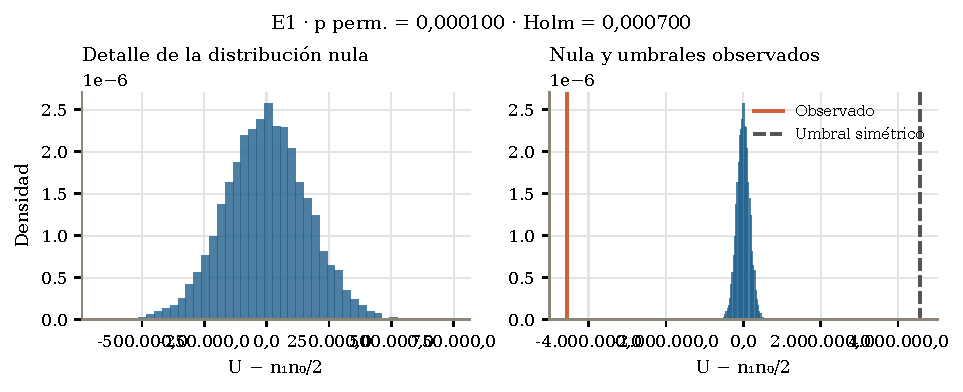
\includegraphics[width=0.85\linewidth,height=0.42\textheight,keepaspectratio]{../../outputs/validacion_completa/figuras/fig_perm_4_e1.pdf}\caption{Distribución nula por permutación: E1, $U$ de Mann--Whitney del peso.}\label{fig:B1}\end{figure}

\begin{figure}[H]\centering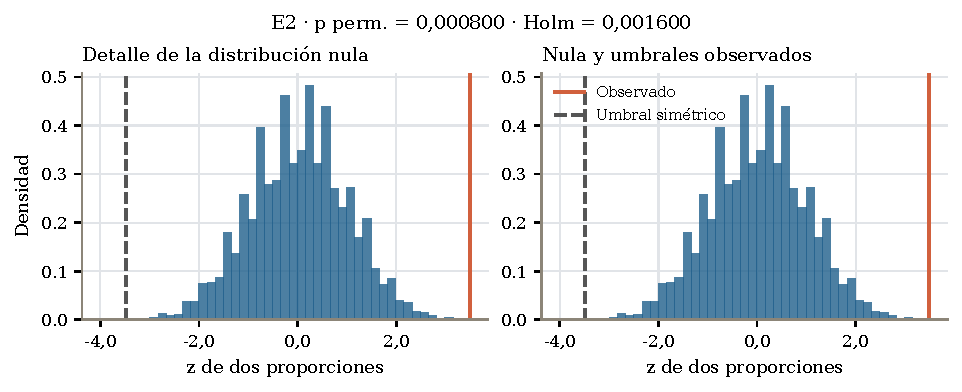
\includegraphics[width=0.85\linewidth,height=0.42\textheight,keepaspectratio]{../../outputs/validacion_completa/figuras/fig_perm_5_e2.pdf}\caption{Distribución nula por permutación: E2, $z$ de dos proporciones (importancia alta / resto).}\label{fig:B2}\end{figure}

\begin{figure}[H]\centering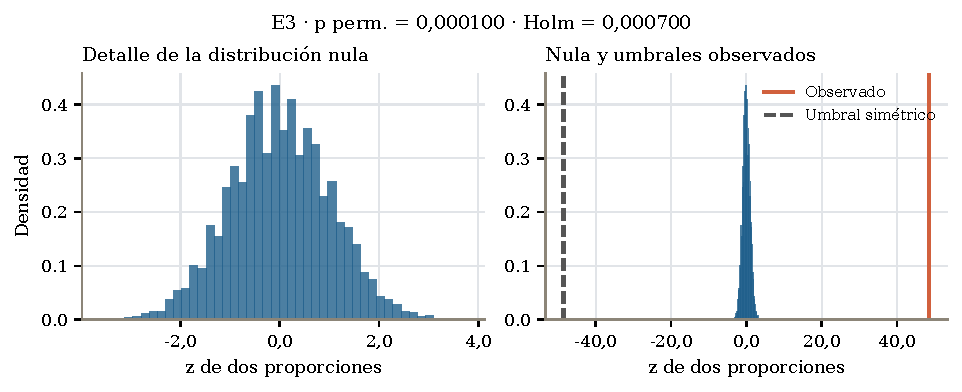
\includegraphics[width=0.85\linewidth,height=0.42\textheight,keepaspectratio]{../../outputs/validacion_completa/figuras/fig_perm_6_e3.pdf}\caption{Distribución nula por permutación: E3, $z$ de dos proporciones (descuento $>$ 10 / $\le$ 10).}\label{fig:B3}\end{figure}

\begin{figure}[H]\centering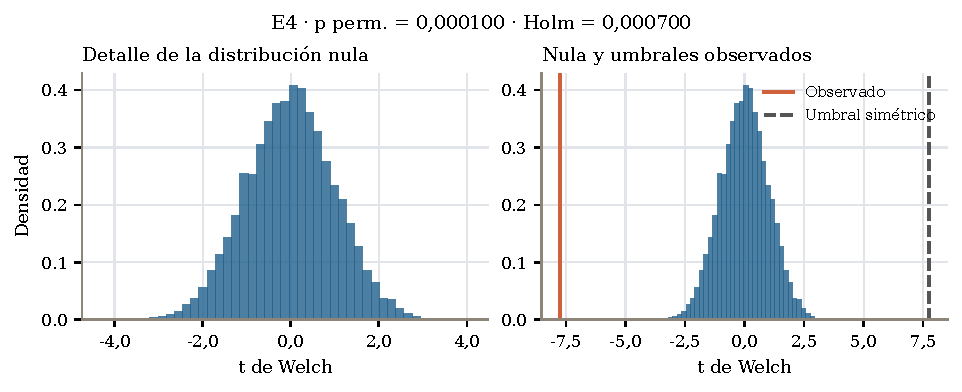
\includegraphics[width=0.85\linewidth,height=0.42\textheight,keepaspectratio]{../../outputs/validacion_completa/figuras/fig_perm_7_e4.pdf}\caption{Distribución nula por permutación: E4, $t$ de Welch del costo.}\label{fig:B4}\end{figure}

\clearpage\section{Anexo C. Las 20 correlaciones y las 15 asociaciones de S1}\label{anx:C}

\setcounter{table}{0}\setcounter{figure}{0}\renewcommand{\thetable}{C-\arabic{table}}\renewcommand{\thefigure}{C-\arabic{figure}}

\emph{Bootstrap} de filas emparejadas con $B = 10.000$ (flujo \texttt{bootstrap\_coeficientes}) e IC percentil al 95\,\%; en Spearman, los rangos se recalculan en cada réplica. Las mismas remuestras sirven para los 35 coeficientes. Para la V de Cramér, acotada en $[0, 1]$, el IC describe magnitud y precisión: un IC positivo no prueba dependencia, porque el estimador está sesgado hacia arriba cerca de cero. Fuentes: \texttt{correlaciones\_bootstrap.csv} y \texttt{asociaciones\_bootstrap.csv}.

{\scriptsize\setlength{\tabcolsep}{3pt}
\begin{longtable}{@{}l l l r r r l r c@{}}
\caption{Las 20 correlaciones de S1 con IC \emph{bootstrap} percentil.}\label{tab:C1}\\\toprule
ID & Coef. & Par & S1 & Sesgo & EE & IC 95\,\% & Ancho & Incluye 0\\\midrule\endfirsthead
\multicolumn{9}{@{}l}{\emph{Continuación de la tabla \ref{tab:C1}}}\\\toprule
ID & Coef. & Par & S1 & Sesgo & EE & IC 95\,\% & Ancho & Incluye 0\\\midrule\endhead
\bottomrule\endfoot
COR-011 & $r_{pb}$ & Compras previas -- Atraso & $-$0,0555 & $-2{,}13\cdot 10^{-4}$ & 0,0096 & [$-$0,075; $-$0,037] & 0,037 & No\\
COR-012 & $r_{pb}$ & Costo -- Atraso & $-$0,0736 & $-3{,}68\cdot 10^{-5}$ & 0,0095 & [$-$0,092; $-$0,055] & 0,038 & No\\
COR-013 & $r_{pb}$ & Descuento -- Atraso & 0,3971 & $1{,}78\cdot 10^{-5}$ & 0,0047 & [0,388; 0,407] & 0,019 & No\\
COR-014 & $r_{pb}$ & Llamadas -- Atraso & $-$0,0671 & $-7{,}24\cdot 10^{-5}$ & 0,0096 & [$-$0,086; $-$0,048] & 0,038 & No\\
COR-015 & $r_{pb}$ & Peso -- Atraso & $-$0,2688 & $-4{,}55\cdot 10^{-5}$ & 0,0092 & [$-$0,287; $-$0,251] & 0,036 & No\\
COR-016 & $\rho$ & Compras previas -- Costo & 0,1942 & $6{,}22\cdot 10^{-5}$ & 0,0091 & [0,176; 0,212] & 0,036 & No\\
COR-017 & $\rho$ & Compras previas -- Descuento & $-$0,0939 & $-5{,}59\cdot 10^{-5}$ & 0,0095 & [$-$0,112; $-$0,075] & 0,037 & No\\
COR-018 & $\rho$ & Compras previas -- Atraso & $-$0,0746 & $-1{,}74\cdot 10^{-4}$ & 0,0096 & [$-$0,094; $-$0,056] & 0,037 & No\\
COR-019 & $\rho$ & Compras previas -- Llamadas & 0,2730 & $-5{,}26\cdot 10^{-5}$ & 0,0086 & [0,256; 0,290] & 0,034 & No\\
COR-020 & $\rho$ & Compras previas -- Peso & $-$0,2347 & $9{,}01\cdot 10^{-5}$ & 0,0092 & [$-$0,253; $-$0,216] & 0,036 & No\\
COR-021 & $\rho$ & Costo -- Descuento & $-$0,1158 & $-5{,}81\cdot 10^{-5}$ & 0,0093 & [$-$0,134; $-$0,098] & 0,037 & No\\
COR-022 & $\rho$ & Costo -- Atraso & $-$0,0719 & $-3{,}25\cdot 10^{-5}$ & 0,0095 & [$-$0,090; $-$0,053] & 0,037 & No\\
COR-023 & $\rho$ & Costo -- Llamadas & 0,2937 & $7{,}35\cdot 10^{-5}$ & 0,0095 & [0,275; 0,312] & 0,037 & No\\
COR-024 & $\rho$ & Costo -- Peso & $-$0,1320 & $3{,}58\cdot 10^{-5}$ & 0,0102 & [$-$0,152; $-$0,112] & 0,040 & No\\
COR-025 & $\rho$ & Descuento -- Atraso & 0,3351 & $-8{,}14\cdot 10^{-5}$ & 0,0083 & [0,319; 0,351] & 0,033 & No\\
COR-026 & $\rho$ & Descuento -- Llamadas & $-$0,1042 & $8{,}66\cdot 10^{-5}$ & 0,0095 & [$-$0,123; $-$0,085] & 0,037 & No\\
COR-027 & $\rho$ & Descuento -- Peso & $-$0,3157 & $9{,}76\cdot 10^{-5}$ & 0,0087 & [$-$0,333; $-$0,298] & 0,034 & No\\
COR-028 & $\rho$ & Llamadas -- Atraso & $-$0,0643 & $-6{,}97\cdot 10^{-5}$ & 0,0096 & [$-$0,083; $-$0,046] & 0,037 & No\\
COR-029 & $\rho$ & Llamadas -- Peso & $-$0,2329 & $2{,}96\cdot 10^{-5}$ & 0,0095 & [$-$0,252; $-$0,214] & 0,037 & No\\
COR-030 & $\rho$ & Peso -- Atraso & $-$0,2660 & $-1{,}80\cdot 10^{-5}$ & 0,0093 & [$-$0,284; $-$0,248] & 0,036 & No\\
\end{longtable}}

{\scriptsize\setlength{\tabcolsep}{3pt}
\begin{longtable}{@{}l l r r r r l r@{}}
\caption{Las 15 asociaciones V de Cramér de S1 con IC \emph{bootstrap} percentil.}\label{tab:C2}\\\toprule
ID & Par & V S1 & Media boot. & Sesgo & EE & IC 95\,\% & Ancho\\\midrule\endfirsthead
\multicolumn{8}{@{}l}{\emph{Continuación de la tabla \ref{tab:C2}}}\\\toprule
ID & Par & V S1 & Media boot. & Sesgo & EE & IC 95\,\% & Ancho\\\midrule\endhead
\bottomrule\endfoot
ASO-001 & Bodega -- Calificación & 0,0151 & 0,0240 & 0,0089 & 0,0039 & [0,017; 0,032] & 0,015\\
ASO-002 & Bodega -- Atraso & 0,0100 & 0,0202 & 0,0103 & 0,0072 & [0,008; 0,036] & 0,028\\
ASO-003 & Bodega -- Género & 0,0087 & 0,0197 & 0,0111 & 0,0070 & [0,008; 0,034] & 0,027\\
ASO-004 & Bodega -- Importancia & 0,0191 & 0,0265 & 0,0074 & 0,0058 & [0,016; 0,038] & 0,023\\
ASO-005 & Bodega -- Modalidad & 0,0011 & 0,0186 & 0,0175 & 0,0047 & [0,010; 0,028] & 0,018\\
ASO-006 & Calificación -- Atraso & 0,0171 & 0,0243 & 0,0072 & 0,0080 & [0,009; 0,041] & 0,031\\
ASO-007 & Calificación -- Género & 0,0164 & 0,0239 & 0,0075 & 0,0080 & [0,009; 0,041] & 0,031\\
ASO-008 & Calificación -- Importancia & 0,0181 & 0,0256 & 0,0075 & 0,0057 & [0,015; 0,037] & 0,022\\
ASO-009 & Calificación -- Modalidad & 0,0170 & 0,0250 & 0,0079 & 0,0056 & [0,015; 0,036] & 0,022\\
ASO-010 & Género -- Atraso & 0,0047 & 0,0086 & 0,0039 & 0,0064 & [0,000; 0,024] & 0,023\\
ASO-011 & Género -- Importancia & 0,0100 & 0,0151 & 0,0051 & 0,0075 & [0,003; 0,031] & 0,029\\
ASO-012 & Género -- Modalidad & 0,0182 & 0,0210 & 0,0028 & 0,0087 & [0,005; 0,039] & 0,034\\
ASO-013 & Importancia -- Atraso & 0,0333 & 0,0348 & 0,0015 & 0,0092 & [0,017; 0,053] & 0,036\\
ASO-014 & Importancia -- Modalidad & 0,0100 & 0,0158 & 0,0058 & 0,0055 & [0,006; 0,028] & 0,022\\
ASO-015 & Modalidad -- Atraso & 0,0082 & 0,0140 & 0,0058 & 0,0071 & [0,003; 0,029] & 0,027\\
\end{longtable}}
{\footnotesize El sesgo positivo en las V cercanas a cero es esperable: la V remuestreada nunca es negativa. Las asociaciones con el atraso (T01 incluida) se validan una vez y se referencian desde el Anexo B.\par}\medskip

\begin{figure}[H]\centering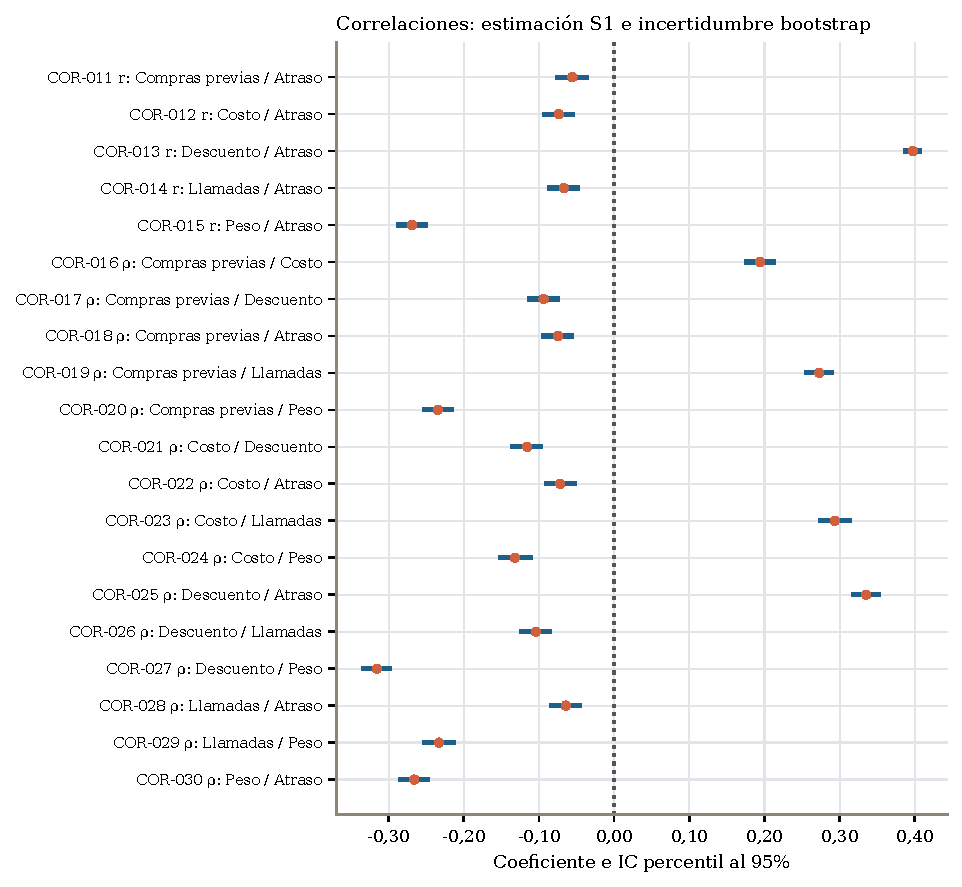
\includegraphics[width=\linewidth,height=0.42\textheight,keepaspectratio]{../../outputs/validacion_completa/figuras/fig_cor_correlaciones_intervalos.pdf}\caption{IC \emph{bootstrap} de las 20 correlaciones de S1.}\label{fig:C1}\end{figure}

\begin{figure}[H]\centering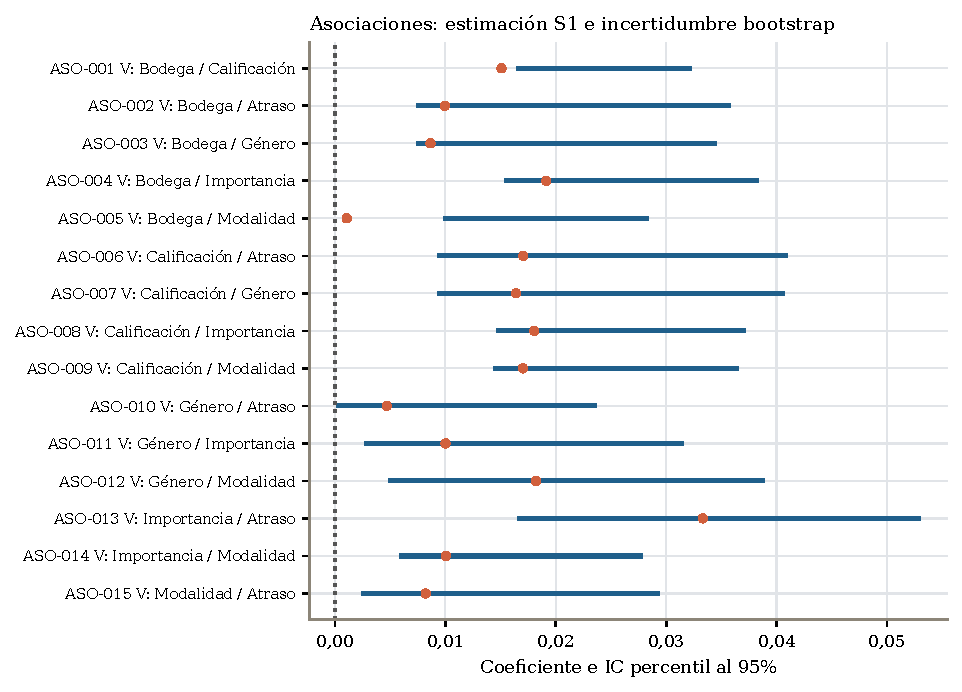
\includegraphics[width=\linewidth,height=0.42\textheight,keepaspectratio]{../../outputs/validacion_completa/figuras/fig_cor_asociaciones_intervalos.pdf}\caption{IC \emph{bootstrap} de las 15 asociaciones V de Cramér.}\label{fig:C2}\end{figure}

\clearpage\section{Anexo D. Simulación Monte Carlo ampliada}\label{anx:D}

\setcounter{table}{0}\setcounter{figure}{0}\renewcommand{\thetable}{D-\arabic{table}}\renewcommand{\thefigure}{D-\arabic{figure}}

Las tablas D-1 a D-4 provienen del notebook de validación completa, cuyo flujo aleatorio se consume en otro orden que en el de entrega; por eso algunas cifras difieren en el último decimal respecto del cuerpo. Todas usan $p = 6.563/10.999$ o valores del IC de Wilson de S1 y $B = 10.000$ lotes.

{\scriptsize\setlength{\tabcolsep}{3pt}
\begin{longtable}{@{}r r r r l r r r r r r c@{}}
\caption{Lotes binomiales por tamaño: estadísticos simulados frente a los exactos.}\label{tab:D1}\\\toprule
$N$ & Media & DE & DE exacta & Rango 95\,\% & P99 & P99 exacto & P($>$0,6) & Exacta & MCSE med. & MCSE prob. & Tol.\\\midrule\endfirsthead
\multicolumn{12}{@{}l}{\emph{Continuación de la tabla \ref{tab:D1}}}\\\toprule
$N$ & Media & DE & DE exacta & Rango 95\,\% & P99 & P99 exacto & P($>$0,6) & Exacta & MCSE med. & MCSE prob. & Tol.\\\midrule\endhead
\bottomrule\endfoot
100 & 0,5970 & 0,0491 & 0,0491 & [0,500; 0,690] & 0,710 & 0,710 & 0,4360 & 0,4353 & 0,00049 & 0,0050 & Sí\\
500 & 0,5968 & 0,0218 & 0,0219 & [0,554; 0,640] & 0,648 & 0,648 & 0,4207 & 0,4233 & 0,00022 & 0,0049 & Sí\\
1.000 & 0,5966 & 0,0155 & 0,0155 & [0,566; 0,627] & 0,633 & 0,633 & 0,3980 & 0,4038 & 0,00015 & 0,0049 & Sí\\
5.000 & 0,5967 & 0,0069 & 0,0069 & [0,583; 0,611] & 0,613 & 0,613 & 0,3106 & 0,3118 & 0,00007 & 0,0046 & Sí\\
\end{longtable}}
{\footnotesize Tolerancias fijadas antes de ejecutar: MCSE de la media $\le 0{,}001$ y de la probabilidad $\le 0{,}005$.\par}\medskip

{\scriptsize\setlength{\tabcolsep}{3pt}
\begin{longtable}{@{}r r r r r r r r@{}}
\caption{Convergencia de la media y de P(tasa $> 60$\,\%) según el número de lotes simulados.}\label{tab:D2}\\\toprule
$N$ & $B$ parcial & Media & MCSE media & P($>$0,6) & MCSE prob. & Dif. media & Dif. prob.\\\midrule\endfirsthead
\multicolumn{8}{@{}l}{\emph{Continuación de la tabla \ref{tab:D2}}}\\\toprule
$N$ & $B$ parcial & Media & MCSE media & P($>$0,6) & MCSE prob. & Dif. media & Dif. prob.\\\midrule\endhead
\bottomrule\endfoot
100 & 100 & 0,5980 & 0,00508 & 0,4400 & 0,0496 & 0,00131 & 0,0047\\
100 & 500 & 0,5950 & 0,00226 & 0,4140 & 0,0220 & $-$0,00171 & $-$0,0213\\
100 & 1.000 & 0,5966 & 0,00161 & 0,4340 & 0,0157 & $-$0,00011 & $-$0,0013\\
100 & 5.000 & 0,5969 & 0,00069 & 0,4312 & 0,0070 & 0,00019 & $-$0,0041\\
100 & 10.000 & 0,5970 & 0,00049 & 0,4360 & 0,0050 & 0,00033 & 0,0007\\
500 & 100 & 0,5983 & 0,00237 & 0,4300 & 0,0495 & 0,00165 & 0,0067\\
500 & 500 & 0,5961 & 0,00101 & 0,4100 & 0,0220 & $-$0,00064 & $-$0,0133\\
500 & 1.000 & 0,5964 & 0,00070 & 0,4240 & 0,0156 & $-$0,00029 & 0,0007\\
500 & 5.000 & 0,5968 & 0,00031 & 0,4220 & 0,0070 & 0,00011 & $-$0,0013\\
500 & 10.000 & 0,5968 & 0,00022 & 0,4207 & 0,0049 & 0,00008 & $-$0,0026\\
1.000 & 100 & 0,5958 & 0,00167 & 0,4200 & 0,0494 & $-$0,00090 & 0,0162\\
1.000 & 500 & 0,5957 & 0,00072 & 0,3920 & 0,0218 & $-$0,00102 & $-$0,0118\\
1.000 & 1.000 & 0,5961 & 0,00050 & 0,4020 & 0,0155 & $-$0,00061 & $-$0,0018\\
1.000 & 5.000 & 0,5965 & 0,00022 & 0,3930 & 0,0069 & $-$0,00019 & $-$0,0108\\
1.000 & 10.000 & 0,5966 & 0,00015 & 0,3980 & 0,0049 & $-$0,00005 & $-$0,0058\\
5.000 & 100 & 0,5981 & 0,00066 & 0,4000 & 0,0490 & 0,00140 & 0,0882\\
5.000 & 500 & 0,5968 & 0,00030 & 0,3200 & 0,0209 & 0,00014 & 0,0082\\
5.000 & 1.000 & 0,5969 & 0,00022 & 0,3330 & 0,0149 & 0,00021 & 0,0212\\
5.000 & 5.000 & 0,5967 & 0,00010 & 0,3098 & 0,0065 & 0,00003 & $-$0,0020\\
5.000 & 10.000 & 0,5967 & 0,00007 & 0,3106 & 0,0046 & $-$0,00000 & $-$0,0012\\
\end{longtable}}
{\footnotesize Dif.: valor simulado menos valor binomial exacto.\par}\medskip

{\scriptsize\setlength{\tabcolsep}{3pt}
\begin{longtable}{@{}r r r r r r r r r r@{}}
\caption{Modelo de dos segmentos (descuento $> 10$ con tasa 1; resto con tasa $3.916/8.352$) frente al modelo homogéneo.}\label{tab:D3}\\\toprule
$N$ & $N_{alto}$ & Media & DE & DE homog. & Razón DE & P99 & P($>$0,6) & Exacta & Homog.\\\midrule\endfirsthead
\multicolumn{10}{@{}l}{\emph{Continuación de la tabla \ref{tab:D3}}}\\\toprule
$N$ & $N_{alto}$ & Media & DE & DE homog. & Razón DE & P99 & P($>$0,6) & Exacta & Homog.\\\midrule\endhead
\bottomrule\endfoot
100 & 24 & 0,5963 & 0,0436 & 0,0491 & 0,888 & 0,700 & 0,4226 & 0,4203 & 0,4360\\
500 & 120 & 0,5967 & 0,0197 & 0,0218 & 0,903 & 0,644 & 0,4154 & 0,4050 & 0,4207\\
1.000 & 241 & 0,5967 & 0,0138 & 0,0155 & 0,890 & 0,629 & 0,3925 & 0,3957 & 0,3980\\
5.000 & 1.203 & 0,5966 & 0,0061 & 0,0069 & 0,885 & 0,611 & 0,2838 & 0,2879 & 0,3106\\
\end{longtable}}
{\footnotesize $N_{alto} = \mathrm{redondeo}(N \cdot 2.647/10.999)$. La tasa 1 del segmento alto es una frontera muestral, no una certeza poblacional.\par}\medskip

{\scriptsize\setlength{\tabcolsep}{3pt}
\begin{longtable}{@{}l l r r r r r r r@{}}
\caption{Sensibilidad del Monte Carlo a las entradas con IC en S1 (extremos y centro del IC).}\label{tab:D4}\\\toprule
Entrada & Escenario & Valor & $N$ & Media & P99 & P($>$0,6) & Exacta & MCSE prob.\\\midrule\endfirsthead
\multicolumn{9}{@{}l}{\emph{Continuación de la tabla \ref{tab:D4}}}\\\toprule
Entrada & Escenario & Valor & $N$ & Media & P99 & P($>$0,6) & Exacta & MCSE prob.\\\midrule\endhead
\bottomrule\endfoot
proporcion\_atraso & Wilson inferior & 0,5875 & 1.000 & 0,5875 & 0,624 & 0,2030 & 0,2018 & 0,0040\\
proporcion\_atraso & Estimación S1 & 0,5967 & 1.000 & 0,5967 & 0,633 & 0,4067 & 0,4038 & 0,0049\\
proporcion\_atraso & Wilson superior & 0,6058 & 1.000 & 0,6059 & 0,642 & 0,6330 & 0,6355 & 0,0048\\
peso\_gramos & IC t inferior & 3.603,5 & 1.000 & 3.603,7 & 3.721,212 & --- & --- & ---\\
peso\_gramos & Estimación S1 & 3.634,0 & 1.000 & 3.634,3 & 3.751,778 & --- & --- & ---\\
peso\_gramos & IC t superior & 3.664,6 & 1.000 & 3.664,9 & 3.782,344 & --- & --- & ---\\
costo\_producto & IC t inferior & 209,30 & 1.000 & 209,28 & 212,744 & --- & --- & ---\\
costo\_producto & Estimación S1 & 210,20 & 1.000 & 210,18 & 213,642 & --- & --- & ---\\
costo\_producto & IC t superior & 211,10 & 1.000 & 211,08 & 214,540 & --- & --- & ---\\
llamadas\_atencion & IC t inferior & 4,0331 & 1.000 & 4,0334 & 4,120 & --- & --- & ---\\
llamadas\_atencion & Estimación S1 & 4,0545 & 1.000 & 4,0548 & 4,141 & --- & --- & ---\\
llamadas\_atencion & IC t superior & 4,0758 & 1.000 & 4,0761 & 4,162 & --- & --- & ---\\
\end{longtable}}

\textbf{Extensión Monte Carlo a todos los estimandos.} Según la planificación, cada estimando del inventario se evalúa con remuestras conjuntas de la distribución empírica de S1. Se reutilizan las réplicas \emph{bootstrap} (Anexos A y C) y las distribuciones de permutación (Anexo B), identificadas como experimento Monte Carlo y no como evidencia independiente. La tabla \ref{tab:D5} resume el sesgo relativo y el MCSE por familia; el detalle de los 194 resultados está en \texttt{montecarlo\_empirico.csv} y en la figura \ref{fig:D1}.

{\scriptsize\setlength{\tabcolsep}{3pt}
\begin{longtable}{@{}l r r r r r@{}}
\caption{Monte Carlo sobre la distribución empírica: sesgo relativo respecto del valor de S1, por familia.}\label{tab:D5}\\\toprule
Familia & Resultados & Con sesgo definido & |Sesgo rel.| mediano (\%) & |Sesgo rel.| máx. (\%) & MCSE máx. de la media\\\midrule\endfirsthead
\multicolumn{6}{@{}l}{\emph{Continuación de la tabla \ref{tab:D5}}}\\\toprule
Familia & Resultados & Con sesgo definido & |Sesgo rel.| mediano (\%) & |Sesgo rel.| máx. (\%) & MCSE máx. de la media\\\midrule\endhead
\bottomrule\endfoot
asociaciones & 15 & 15 & 105,147 & 374,227 & $9{,}18\cdot 10^{-5}$\\
correlaciones & 30 & 20 & 0,653 & 2,223 & $1{,}02\cdot 10^{-4}$\\
descriptivas & 111 & 88 & 1,316 & 79,844 & 1,4516\\
efectos & 13 & 13 & 0,736 & 2,052 & 0,3064\\
parametros & 4 & 4 & 0,635 & 1,349 & 0,1554\\
pruebas & 21 & 0 & --- & --- & ---\\
\end{longtable}}
{\footnotesize Sin sesgo definido: distribuciones nulas de permutación, $p$ ajustados por Holm, $p$ de correlación (evaluados con su coeficiente) y extremos muestrales.\par}\medskip

\begin{figure}[H]\centering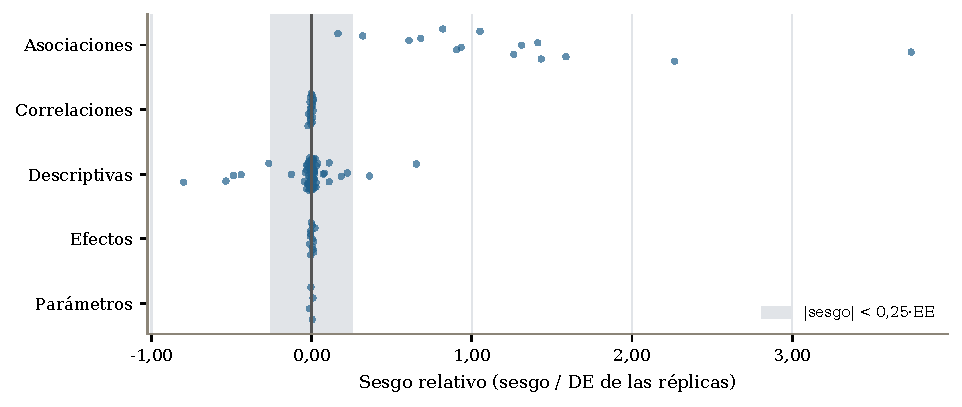
\includegraphics[width=\linewidth,height=0.42\textheight,keepaspectratio]{../../outputs/validacion_completa/figuras/fig_mc_D01_sesgo_relativo.pdf}\caption{Sesgo relativo Monte Carlo de cada estimando respecto de su valor empírico.}\label{fig:D1}\end{figure}

\clearpage\section{Anexo E. Robustez: \emph{jackknife}, influencia y escenarios}\label{anx:E}

\setcounter{table}{0}\setcounter{figure}{0}\renewcommand{\thetable}{E-\arabic{table}}\renewcommand{\thefigure}{E-\arabic{figure}}

\textbf{\emph{Jackknife}.} Se recalcula cada uno de los 194 resultados del inventario retirando, uno a la vez, cada envío; en los efectos por grupo se conserva la pertenencia y se actualizan los tamaños. Los 24 resultados ``no aplica'' son valores $p$: los de las pruebas se evalúan como cambio de decisión (cruda y Holm) y los de correlación, a través de su coeficiente. Los diez envíos más influyentes de cada resultado, con su valor original y el cambio absoluto y relativo, están en \texttt{jackknife\_influyentes.csv} (1.700 filas; los empates se resuelven por \texttt{id\_envio}).

{\tiny\setlength{\tabcolsep}{3pt}
\begin{longtable}{@{}l >{\raggedright\arraybackslash}p{2.6cm} >{\raggedright\arraybackslash}p{2.2cm} r r r r r c@{}}
\caption{\emph{Jackknife} de los 194 resultados de S1: EE y mayor cambio al retirar un envío.}\label{tab:E1}\\\toprule
ID & Estimando & Grupo & Estimación & EE \emph{jk} & Cambio máx. & Cambio rel. (\%) & Envío & Cambian dec.\\\midrule\endfirsthead
\multicolumn{9}{@{}l}{\emph{Continuación de la tabla \ref{tab:E1}}}\\\toprule
ID & Estimando & Grupo & Estimación & EE \emph{jk} & Cambio máx. & Cambio rel. (\%) & Envío & Cambian dec.\\\midrule\endhead
\bottomrule\endfoot
PAR-001 & Media, costo & global & 210,20 & 0,4583 & 0,0104 & 0,0049 & 432 & \\
PAR-002 & Media, llamadas & global & 4,0545 & 0,0109 & $2{,}68\cdot 10^{-4}$ & 0,0066 & 266 & \\
PAR-003 & Media, peso & global & 3.634,0 & 15,59 & 0,3830 & 0,0105 & 200 & \\
PAR-004 & Proporción, atraso & 1 & 0,5967 & 0,0047 & $5{,}43\cdot 10^{-5}$ & 0,0091 & 3.136 & \\
EFE-001 & $d_{av}$, compras previas & atras. $-$ punt. & $-$0,1133 & 0,0194 & $8{,}35\cdot 10^{-4}$ & 0,7369 & 3.154 & \\
EFE-002 & $d_{av}$, costo & atras. $-$ punt. & $-$0,1505 & 0,0195 & $5{,}96\cdot 10^{-4}$ & 0,3959 & 7.930 & \\
EFE-003 & $d_{av}$, descuento & atras. $-$ punt. & 0,9600 & 0,0124 & $2{,}30\cdot 10^{-4}$ & 0,0240 & 110 & \\
EFE-004 & $d_{av}$, llamadas & atras. $-$ punt. & $-$0,1367 & 0,0195 & $5{,}23\cdot 10^{-4}$ & 0,3826 & 3.605 & \\
EFE-005 & $d_{av}$, peso & atras. $-$ punt. & $-$0,5689 & 0,0212 & $6{,}04\cdot 10^{-4}$ & 0,1061 & 200 & \\
EFE-006 & Dif. de medias, costo & atras. $-$ punt. & $-$7,2095 & 0,9306 & 0,0265 & 0,3675 & 7.930 & \\
EFE-007 & Dif. de medias, descuento & atras. $-$ punt. & 13,12 & 0,2398 & 0,0071 & 0,0538 & 112 & \\
EFE-008 & Dif. de medias, peso & atras. $-$ punt. & $-$896,03 & 30,61 & 0,7142 & 0,0797 & 6.034 & \\
EFE-009 & Dif. de proporciones, descuento & Descuento $>$ 10 - Descuento $\le$ 10 & 0,5311 & 0,0055 & $6{,}36\cdot 10^{-5}$ & 0,0120 & 4 & \\
EFE-010 & Dif. de proporciones, importancia & Importancia=alta - Importancia en \{baja, media\} & 0,0581 & 0,0163 & $6{,}86\cdot 10^{-4}$ & 1,1809 & 3.138 & \\
EFE-011 & Biserial de rangos, peso & atras. $-$ punt. & $-$0,3130 & 0,0109 & $2{,}96\cdot 10^{-4}$ & 0,0946 & 6.034 & \\
EFE-012 & Riesgo relativo, descuento & Descuento $>$ 10 / Descuento $\le$ 10 & 2,1328 & 0,0248 & $2{,}89\cdot 10^{-4}$ & 0,0136 & 4 & \\
EFE-013 & Riesgo relativo, importancia & Importancia=alta / Importancia en \{baja, media\} & 1,0982 & 0,0277 & 0,0012 & 0,1056 & 3.138 & \\
DES-001 & Asimetría, compras previas & global & 1,6819 & 0,0313 & 0,0017 & 0,1006 & 183 & \\
DES-002 & Asimetría, costo & global & $-$0,1571 & 0,0152 & $4{,}58\cdot 10^{-4}$ & 0,2918 & 432 & \\
DES-003 & Asimetría, descuento & global & 1,7989 & 0,0289 & $7{,}38\cdot 10^{-4}$ & 0,0410 & 2.751 & \\
DES-004 & Asimetría, llamadas & global & 0,3919 & 0,0167 & $5{,}21\cdot 10^{-4}$ & 0,1330 & 8.264 & \\
DES-005 & Asimetría, peso & global & $-$0,2497 & 0,0159 & 0,0011 & 0,4272 & 200 & \\
DES-006 & Curtosis (exceso), compras previas & global & 4,0063 & 0,1370 & 0,0054 & 0,1351 & 8.285 & \\
DES-007 & Curtosis (exceso), costo & global & $-$0,9722 & 0,0165 & $8{,}67\cdot 10^{-4}$ & 0,0892 & 432 & \\
DES-008 & Curtosis (exceso), descuento & global & 2,0006 & 0,1220 & 0,0033 & 0,1669 & 62 & \\
DES-009 & Curtosis (exceso), llamadas & global & $-$0,3090 & 0,0289 & $6{,}53\cdot 10^{-4}$ & 0,2114 & 8.264 & \\
DES-010 & Curtosis (exceso), peso & global & $-$1,4477 & 0,0136 & 0,0025 & 0,1733 & 200 & \\
DES-011 & DE, compras previas & global & 1,5229 & 0,0178 & 0,0012 & 0,0766 & 2.761 & \\
DES-012 & DE, costo & atrasada & 48,05 & 0,2947 & 0,0160 & 0,0333 & 432 & \\
DES-013 & DE, costo & global & 48,06 & 0,2323 & 0,0102 & 0,0211 & 432 & \\
DES-014 & DE, costo & puntual & 47,76 & 0,3783 & 0,0272 & 0,0570 & 7.930 & \\
DES-015 & DE, descuento & atrasada & 19,11 & 0,1524 & 0,0071 & 0,0372 & 112 & \\
DES-016 & DE, descuento & global & 16,21 & 0,1545 & 0,0067 & 0,0416 & 112 & \\
DES-017 & DE, descuento & puntual & 2,8777 & 0,0190 & $4{,}86\cdot 10^{-4}$ & 0,0169 & 3.146 & \\
DES-018 & DE, llamadas & global & 1,1415 & 0,0071 & $2{,}94\cdot 10^{-4}$ & 0,0257 & 266 & \\
DES-019 & DE, peso & atrasada & 1.576,1 & 7,6547 & 0,8916 & 0,0566 & 200 & \\
DES-020 & DE, peso & global & 1.635,4 & 5,7958 & 0,4190 & 0,0256 & 200 & \\
DES-021 & DE, peso & puntual & 1.574,0 & 13,77 & 0,5417 & 0,0344 & 6.034 & \\
DES-022 & IQR, compras previas & global & 1,0000 & 0 & 0 & 0,0000 & 1 & \\
DES-023 & IQR, costo & global & 82,00 & 11,35 & 0,2500 & 0,3049 & 6 & \\
DES-024 & IQR, descuento & global & 6,0000 & 0 & 0 & 0,0000 & 1 & \\
DES-025 & IQR, llamadas & global & 2,0000 & 0 & 0 & 0,0000 & 1 & \\
DES-026 & IQR, peso & global & 3.210,5 & 32,11 & 0,5000 & 0,0156 & 1 & \\
DES-027 & Máximo, compras previas & global & 10,00 & 0 & 0 & 0,0000 & 1 & \\
DES-028 & Máximo, costo & global & 310,00 & 0 & 0 & 0,0000 & 1 & \\
DES-029 & Máximo, descuento & global & 65,00 & 0 & 0 & 0,0000 & 1 & \\
DES-030 & Máximo, llamadas & global & 7,0000 & 0 & 0 & 0,0000 & 1 & \\
DES-031 & Máximo, peso & global & 7.846,0 & 161,99 & 162,00 & 2,0647 & 200 & \\
DES-032 & Media, compras previas & atrasada & 3,4981 & 0,0187 & $9{,}91\cdot 10^{-4}$ & 0,0283 & 183 & \\
DES-033 & Media, compras previas & global & 3,5676 & 0,0145 & $5{,}85\cdot 10^{-4}$ & 0,0164 & 183 & \\
DES-034 & Media, compras previas & puntual & 3,6704 & 0,0229 & 0,0014 & 0,0389 & 3.154 & \\
DES-035 & Media, costo & atrasada & 207,29 & 0,5932 & 0,0170 & 0,0082 & 432 & \\
DES-036 & Media, costo & puntual & 214,50 & 0,7170 & 0,0265 & 0,0124 & 7.930 & \\
DES-037 & Media, descuento & atrasada & 18,66 & 0,2359 & 0,0071 & 0,0378 & 112 & \\
DES-038 & Media, descuento & global & 13,37 & 0,1545 & 0,0047 & 0,0351 & 112 & \\
DES-039 & Media, descuento & puntual & 5,5460 & 0,0432 & 0,0010 & 0,0185 & 3.146 & \\
DES-040 & Media, llamadas & atrasada & 3,9915 & 0,0139 & $4{,}58\cdot 10^{-4}$ & 0,0115 & 266 & \\
DES-041 & Media, llamadas & puntual & 4,1477 & 0,0175 & $6{,}43\cdot 10^{-4}$ & 0,0155 & 3.605 & \\
DES-042 & Media, peso & atrasada & 3.272,6 & 19,46 & 0,6969 & 0,0213 & 200 & \\
DES-043 & Media, peso & puntual & 4.168,7 & 23,63 & 0,7142 & 0,0171 & 6.034 & \\
DES-044 & Mediana, compras previas & atrasada & 3,0000 & 0 & 0 & 0,0000 & 1 & \\
DES-045 & Mediana, compras previas & global & 3,0000 & 0 & 0 & 0,0000 & 1 & \\
DES-046 & Mediana, compras previas & puntual & 3,0000 & 0 & 0 & 0,0000 & 1 & \\
DES-047 & Mediana, costo & atrasada & 209,00 & 0 & 0 & 0,0000 & 1 & \\
DES-048 & Mediana, costo & global & 214,00 & 0 & 0 & 0,0000 & 1 & \\
DES-049 & Mediana, costo & puntual & 222,00 & 0 & 0 & 0,0000 & 1 & \\
DES-050 & Mediana, descuento & atrasada & 9,0000 & 0 & 0 & 0,0000 & 1 & \\
DES-051 & Mediana, descuento & global & 7,0000 & 0 & 0 & 0,0000 & 1 & \\
DES-052 & Mediana, descuento & puntual & 6,0000 & 0 & 0 & 0,0000 & 1 & \\
DES-053 & Mediana, llamadas & atrasada & 4,0000 & 0 & 0 & 0,0000 & 1 & \\
DES-054 & Mediana, llamadas & global & 4,0000 & 0 & 0 & 0,0000 & 1 & \\
DES-055 & Mediana, llamadas & puntual & 4,0000 & 0 & 0 & 0,0000 & 1 & \\
DES-056 & Mediana, peso & atrasada & 3.231,0 & 0 & 0 & 0,0000 & 1 & \\
DES-057 & Mediana, peso & global & 4.149,0 & 0 & 0 & 0,0000 & 1 & \\
DES-058 & Mediana, peso & puntual & 4.674,0 & 133,19 & 2,0000 & 0,0428 & 3.136 & \\
DES-059 & Mínimo, compras previas & global & 2,0000 & 0 & 0 & 0,0000 & 1 & \\
DES-060 & Mínimo, costo & global & 96,00 & 0 & 0 & 0,0000 & 1 & \\
DES-061 & Mínimo, descuento & global & 1,0000 & 0 & 0 & 0,0000 & 1 & \\
DES-062 & Mínimo, llamadas & global & 2,0000 & 0 & 0 & 0,0000 & 1 & \\
DES-063 & Mínimo, peso & global & 1.001,0 & 0 & 0 & 0,0000 & 1 & \\
DES-064 & Extremos IQR (\%), costo & global & 0 & 0 & 0 & --- & 1 & \\
DES-065 & Extremos IQR (\%), llamadas & global & 0 & 0 & 0 & --- & 1 & \\
DES-066 & Extremos IQR (\%), peso & global & 0 & 0 & 0 & --- & 1 & \\
DES-067 & \% suma top 1\%, costo & global & 1,4485 & 0,0033 & $1{,}90\cdot 10^{-4}$ & 0,0132 & 5.262 & \\
DES-068 & \% suma top 1\%, llamadas & global & 1,7110 & 0,0046 & $2{,}69\cdot 10^{-4}$ & 0,0157 & 266 & \\
DES-069 & \% suma top 1\%, peso & global & 1,6538 & 0,0115 & 0,0044 & 0,2650 & 200 & \\
DES-070 & Proporción, bodega & A & 0,1667 & 0,0036 & $7{,}58\cdot 10^{-5}$ & 0,0455 & 3 & \\
DES-071 & Proporción, bodega & B & 0,1667 & 0,0036 & $7{,}58\cdot 10^{-5}$ & 0,0455 & 4 & \\
DES-072 & Proporción, bodega & C & 0,1667 & 0,0036 & $7{,}58\cdot 10^{-5}$ & 0,0455 & 5 & \\
DES-073 & Proporción, bodega & D & 0,1667 & 0,0036 & $7{,}58\cdot 10^{-5}$ & 0,0454 & 1 & \\
DES-074 & Proporción, bodega & F & 0,3333 & 0,0045 & $6{,}06\cdot 10^{-5}$ & 0,0182 & 2 & \\
DES-075 & Proporción, calificación & 1 & 0,2032 & 0,0038 & $7{,}24\cdot 10^{-5}$ & 0,0357 & 6 & \\
DES-076 & Proporción, calificación & 2 & 0,1968 & 0,0038 & $7{,}30\cdot 10^{-5}$ & 0,0371 & 1 & \\
DES-077 & Proporción, calificación & 3 & 0,2036 & 0,0038 & $7{,}24\cdot 10^{-5}$ & 0,0356 & 4 & \\
DES-078 & Proporción, calificación & 4 & 0,1990 & 0,0038 & $7{,}28\cdot 10^{-5}$ & 0,0366 & 7 & \\
DES-079 & Proporción, calificación & 5 & 0,1974 & 0,0038 & $7{,}30\cdot 10^{-5}$ & 0,0370 & 2 & \\
DES-080 & Proporción, atraso & 0 & 0,4033 & 0,0047 & $5{,}43\cdot 10^{-5}$ & 0,0135 & 3.136 & \\
DES-081 & Proporción, género & F & 0,5041 & 0,0048 & $4{,}58\cdot 10^{-5}$ & 0,0091 & 2 & \\
DES-082 & Proporción, género & M & 0,4959 & 0,0048 & $4{,}58\cdot 10^{-5}$ & 0,0092 & 2 & \\
DES-083 & Proporción, importancia & high & 0,0862 & 0,0027 & $8{,}31\cdot 10^{-5}$ & 0,0964 & 14 & \\
DES-084 & Proporción, importancia & low & 0,4816 & 0,0048 & $4{,}71\cdot 10^{-5}$ & 0,0098 & 1 & \\
DES-085 & Proporción, importancia & medium & 0,4322 & 0,0047 & $5{,}16\cdot 10^{-5}$ & 0,0119 & 4 & \\
DES-086 & Proporción, modalidad & Flight & 0,1616 & 0,0035 & $7{,}62\cdot 10^{-5}$ & 0,0472 & 1 & \\
DES-087 & Proporción, modalidad & Road & 0,1600 & 0,0035 & $7{,}64\cdot 10^{-5}$ & 0,0477 & 111 & \\
DES-088 & Proporción, modalidad & Ship & 0,6784 & 0,0045 & $6{,}17\cdot 10^{-5}$ & 0,0091 & 1 & \\
DES-089 & Q1, compras previas & global & 3,0000 & 0 & 0 & 0,0000 & 1 & \\
DES-090 & Q1, costo & global & 169,00 & 11,35 & 0,2500 & 0,1479 & 6 & \\
DES-091 & Q1, descuento & global & 4,0000 & 0 & 0 & 0,0000 & 1 & \\
DES-092 & Q1, llamadas & global & 3,0000 & 0 & 0 & 0,0000 & 1 & \\
DES-093 & Q1, peso & global & 1.839,5 & 34,06 & 0,5000 & 0,0272 & 1 & \\
DES-094 & Q3, compras previas & global & 4,0000 & 0 & 0 & 0,0000 & 1 & \\
DES-095 & Q3, costo & global & 251,00 & 0 & 0 & 0,0000 & 1 & \\
DES-096 & Q3, descuento & global & 10,00 & 0 & 0 & 0,0000 & 1 & \\
DES-097 & Q3, llamadas & global & 5,0000 & 0 & 0 & 0,0000 & 1 & \\
DES-098 & Q3, peso & global & 5.050,0 & 11,35 & 0,2500 & 0,0050 & 199 & \\
DES-099 & Tasa de atraso, bodega & Bodega=A & 0,5865 & 0,0115 & $3{,}20\cdot 10^{-4}$ & 0,0546 & 3.141 & \\
DES-100 & Tasa de atraso, bodega & Bodega=B & 0,6023 & 0,0114 & $3{,}29\cdot 10^{-4}$ & 0,0546 & 3.136 & \\
DES-101 & Tasa de atraso, calificación & Calificación=1 & 0,5875 & 0,0104 & $2{,}63\cdot 10^{-4}$ & 0,0448 & 3.147 & \\
DES-102 & Tasa de atraso, calificación & Calificación=5 & 0,6066 & 0,0105 & $2{,}80\cdot 10^{-4}$ & 0,0461 & 3.136 & \\
DES-103 & Tasa de atraso, descuento & Descuento $\le$ 10 & 0,4689 & 0,0055 & $6{,}36\cdot 10^{-5}$ & 0,0136 & 4 & \\
DES-104 & Tasa de atraso, descuento & Descuento $>$ 10 & 1,0000 & 0 & 0 & 0,0000 & 1 & \\
DES-105 & Tasa de atraso, género & Género=Fem. & 0,5944 & 0,0066 & $1{,}07\cdot 10^{-4}$ & 0,0180 & 3.146 & \\
DES-106 & Tasa de atraso, género & Género=Masc. & 0,5990 & 0,0066 & $1{,}10\cdot 10^{-4}$ & 0,0183 & 3.136 & \\
DES-107 & Tasa de atraso, importancia & Importancia en \{baja, media\} & 0,5917 & 0,0049 & $5{,}89\cdot 10^{-5}$ & 0,0100 & 3.136 & \\
DES-108 & Tasa de atraso, importancia & Importancia=alta & 0,6498 & 0,0155 & $6{,}86\cdot 10^{-4}$ & 0,1056 & 3.138 & \\
DES-109 & Tasa de atraso, importancia & Importancia=media & 0,5905 & 0,0071 & $1{,}24\cdot 10^{-4}$ & 0,0210 & 3.136 & \\
DES-110 & Tasa de atraso, modalidad & Modalidad=Avión & 0,6016 & 0,0116 & $3{,}39\cdot 10^{-4}$ & 0,0563 & 3.147 & \\
DES-111 & Tasa de atraso, modalidad & Modalidad=Carretera & 0,5881 & 0,0117 & $3{,}34\cdot 10^{-4}$ & 0,0569 & 3.136 & \\
PRU-001 & Estadístico, costo & E4 & $-$7,7471 & 1,0061 & 0,0306 & 0,3947 & 7.930 & 0 / 0\\
PRU-002 & Estadístico, descuento & E3 & 48,54 & 0,5284 & 0,0077 & 0,0158 & 1 & 0 / 0\\
PRU-003 & Estadístico, descuento & T03 & 54,70 & 0,7353 & 0,0172 & 0,0314 & 110 & 0 / 0\\
PRU-004 & Estadístico, importancia & E2 & 3,4863 & 0,9766 & 0,0395 & 1,1343 & 3.138 & 0 / 0\\
PRU-005 & Estadístico, modalidad & T01 & 0,7434 & 1,7260 & 0,0417 & 5,6140 & 3.136 & 0 / 0\\
PRU-006 & Estadístico, peso & E1 & 10.000.332,5 & 163.483,7 & 6.562,0 & 0,0656 & 6.034 & 0 / 0\\
PRU-007 & Estadístico, peso & T02 & $-$29,27 & 1,1094 & 0,0286 & 0,0976 & 200 & 0 / 0\\
PRU-008 & $p$, costo & E4 & --- & \multicolumn{5}{l}{\emph{No aplica: p de prueba: se evalúa como cambio de decisión de la prueba}}\\
PRU-009 & $p$, descuento & E3 & --- & \multicolumn{5}{l}{\emph{No aplica: p de prueba: se evalúa como cambio de decisión de la prueba}}\\
PRU-010 & $p$, descuento & T03 & --- & \multicolumn{5}{l}{\emph{No aplica: p de prueba: se evalúa como cambio de decisión de la prueba}}\\
PRU-011 & $p$, importancia & E2 & --- & \multicolumn{5}{l}{\emph{No aplica: p de prueba: se evalúa como cambio de decisión de la prueba}}\\
PRU-012 & $p$, modalidad & T01 & --- & \multicolumn{5}{l}{\emph{No aplica: p de prueba: se evalúa como cambio de decisión de la prueba}}\\
PRU-013 & $p$, peso & E1 & --- & \multicolumn{5}{l}{\emph{No aplica: p de prueba: se evalúa como cambio de decisión de la prueba}}\\
PRU-014 & $p$, peso & T02 & --- & \multicolumn{5}{l}{\emph{No aplica: p de prueba: se evalúa como cambio de decisión de la prueba}}\\
PRU-015 & $p$ Holm, costo & E4 & --- & \multicolumn{5}{l}{\emph{No aplica: p de prueba: se evalúa como cambio de decisión de la prueba}}\\
PRU-016 & $p$ Holm, descuento & E3 & --- & \multicolumn{5}{l}{\emph{No aplica: p de prueba: se evalúa como cambio de decisión de la prueba}}\\
PRU-017 & $p$ Holm, descuento & T03 & --- & \multicolumn{5}{l}{\emph{No aplica: p de prueba: se evalúa como cambio de decisión de la prueba}}\\
PRU-018 & $p$ Holm, importancia & E2 & --- & \multicolumn{5}{l}{\emph{No aplica: p de prueba: se evalúa como cambio de decisión de la prueba}}\\
PRU-019 & $p$ Holm, modalidad & T01 & --- & \multicolumn{5}{l}{\emph{No aplica: p de prueba: se evalúa como cambio de decisión de la prueba}}\\
PRU-020 & $p$ Holm, peso & E1 & --- & \multicolumn{5}{l}{\emph{No aplica: p de prueba: se evalúa como cambio de decisión de la prueba}}\\
PRU-021 & $p$ Holm, peso & T02 & --- & \multicolumn{5}{l}{\emph{No aplica: p de prueba: se evalúa como cambio de decisión de la prueba}}\\
COR-001 & $p$ correlación, compras previas -- atraso & r\_punto\_biserial & --- & \multicolumn{5}{l}{\emph{No aplica: p de correlación: se evalúa a través del coeficiente}}\\
COR-002 & $p$ correlación, compras previas -- atraso & rho\_spearman & --- & \multicolumn{5}{l}{\emph{No aplica: p de correlación: se evalúa a través del coeficiente}}\\
COR-003 & $p$ correlación, costo -- atraso & r\_punto\_biserial & --- & \multicolumn{5}{l}{\emph{No aplica: p de correlación: se evalúa a través del coeficiente}}\\
COR-004 & $p$ correlación, costo -- atraso & rho\_spearman & --- & \multicolumn{5}{l}{\emph{No aplica: p de correlación: se evalúa a través del coeficiente}}\\
COR-005 & $p$ correlación, descuento -- atraso & r\_punto\_biserial & --- & \multicolumn{5}{l}{\emph{No aplica: p de correlación: se evalúa a través del coeficiente}}\\
COR-006 & $p$ correlación, descuento -- atraso & rho\_spearman & --- & \multicolumn{5}{l}{\emph{No aplica: p de correlación: se evalúa a través del coeficiente}}\\
COR-007 & $p$ correlación, llamadas -- atraso & r\_punto\_biserial & --- & \multicolumn{5}{l}{\emph{No aplica: p de correlación: se evalúa a través del coeficiente}}\\
COR-008 & $p$ correlación, llamadas -- atraso & rho\_spearman & --- & \multicolumn{5}{l}{\emph{No aplica: p de correlación: se evalúa a través del coeficiente}}\\
COR-009 & $p$ correlación, peso -- atraso & r\_punto\_biserial & --- & \multicolumn{5}{l}{\emph{No aplica: p de correlación: se evalúa a través del coeficiente}}\\
COR-010 & $p$ correlación, peso -- atraso & rho\_spearman & --- & \multicolumn{5}{l}{\emph{No aplica: p de correlación: se evalúa a través del coeficiente}}\\
COR-011 & $r_{pb}$, compras previas -- atraso & global & $-$0,0555 & 0,0096 & $4{,}19\cdot 10^{-4}$ & 0,7543 & 3.154 & \\
COR-012 & $r_{pb}$, costo -- atraso & global & $-$0,0736 & 0,0095 & $2{,}84\cdot 10^{-4}$ & 0,3861 & 7.930 & \\
COR-013 & $r_{pb}$, descuento -- atraso & global & 0,3971 & 0,0047 & $7{,}98\cdot 10^{-5}$ & 0,0201 & 13 & \\
COR-014 & $r_{pb}$, llamadas -- atraso & global & $-$0,0671 & 0,0096 & $2{,}61\cdot 10^{-4}$ & 0,3883 & 3.605 & \\
COR-015 & $r_{pb}$, peso -- atraso & global & $-$0,2688 & 0,0092 & $2{,}82\cdot 10^{-4}$ & 0,1049 & 200 & \\
COR-016 & $\rho$, compras previas -- costo & global & 0,1942 & 0,0091 & $3{,}29\cdot 10^{-4}$ & 0,1695 & 4.511 & \\
COR-017 & $\rho$, compras previas -- descuento & global & $-$0,0939 & 0,0094 & $3{,}02\cdot 10^{-4}$ & 0,3221 & 1.146 & \\
COR-018 & $\rho$, compras previas -- atraso & global & $-$0,0746 & 0,0095 & $1{,}80\cdot 10^{-4}$ & 0,2405 & 3.154 & \\
COR-019 & $\rho$, compras previas -- llamadas & global & 0,2730 & 0,0087 & $3{,}51\cdot 10^{-4}$ & 0,1287 & 2.068 & \\
COR-020 & $\rho$, compras previas -- peso & global & $-$0,2347 & 0,0092 & $3{,}39\cdot 10^{-4}$ & 0,1444 & 8.587 & \\
COR-021 & $\rho$, costo -- descuento & global & $-$0,1158 & 0,0094 & $2{,}83\cdot 10^{-4}$ & 0,2447 & 5.908 & \\
COR-022 & $\rho$, costo -- atraso & global & $-$0,0719 & 0,0095 & $2{,}06\cdot 10^{-4}$ & 0,2864 & 7.930 & \\
COR-023 & $\rho$, costo -- llamadas & global & 0,2937 & 0,0095 & $3{,}45\cdot 10^{-4}$ & 0,1174 & 8.908 & \\
COR-024 & $\rho$, costo -- peso & global & $-$0,1320 & 0,0102 & $3{,}00\cdot 10^{-4}$ & 0,2275 & 3.016 & \\
COR-025 & $\rho$, descuento -- atraso & global & 0,3351 & 0,0083 & $1{,}73\cdot 10^{-4}$ & 0,0517 & 13 & \\
COR-026 & $\rho$, descuento -- llamadas & global & $-$0,1042 & 0,0093 & $2{,}94\cdot 10^{-4}$ & 0,2817 & 266 & \\
COR-027 & $\rho$, descuento -- peso & global & $-$0,3157 & 0,0087 & $3{,}36\cdot 10^{-4}$ & 0,1063 & 7.179 & \\
COR-028 & $\rho$, llamadas -- atraso & global & $-$0,0643 & 0,0095 & $2{,}00\cdot 10^{-4}$ & 0,3107 & 3.150 & \\
COR-029 & $\rho$, llamadas -- peso & global & $-$0,2329 & 0,0095 & $3{,}26\cdot 10^{-4}$ & 0,1400 & 1.765 & \\
COR-030 & $\rho$, peso -- atraso & global & $-$0,2660 & 0,0093 & $2{,}46\cdot 10^{-4}$ & 0,0924 & 6.034 & \\
ASO-001 & V de Cramér, bodega -- calificación & global & 0,0151 & 0,0047 & $1{,}18\cdot 10^{-4}$ & 0,7797 & 15 & \\
ASO-002 & V de Cramér, bodega -- atraso & global & 0,0100 & 0,0096 & $2{,}29\cdot 10^{-4}$ & 2,2966 & 3.141 & \\
ASO-003 & V de Cramér, bodega -- género & global & 0,0087 & 0,0095 & $1{,}85\cdot 10^{-4}$ & 2,1407 & 10 & \\
ASO-004 & V de Cramér, bodega -- importancia & global & 0,0191 & 0,0067 & $1{,}91\cdot 10^{-4}$ & 0,9989 & 172 & \\
ASO-005 & V de Cramér, bodega -- modalidad & global & 0,0011 & 0,0064 & $2{,}39\cdot 10^{-4}$ & 22,5162 & 115 & \\
ASO-006 & V de Cramér, calificación -- atraso & global & 0,0171 & 0,0095 & $1{,}35\cdot 10^{-4}$ & 0,7894 & 3.136 & \\
ASO-007 & V de Cramér, calificación -- género & global & 0,0164 & 0,0095 & $1{,}53\cdot 10^{-4}$ & 0,9321 & 1 & \\
ASO-008 & V de Cramér, calificación -- importancia & global & 0,0181 & 0,0068 & $1{,}60\cdot 10^{-4}$ & 0,8873 & 167 & \\
ASO-009 & V de Cramér, calificación -- modalidad & global & 0,0170 & 0,0066 & $2{,}41\cdot 10^{-4}$ & 1,4149 & 4 & \\
ASO-010 & V de Cramér, género -- atraso & global & 0,0047 & 0,0095 & $1{,}12\cdot 10^{-4}$ & 2,3899 & 3.136 & \\
ASO-011 & V de Cramér, género -- importancia & global & 0,0100 & 0,0095 & $1{,}55\cdot 10^{-4}$ & 1,5507 & 27 & \\
ASO-012 & V de Cramér, género -- modalidad & global & 0,0182 & 0,0095 & $1{,}93\cdot 10^{-4}$ & 1,0617 & 1 & \\
ASO-013 & V de Cramér, importancia -- atraso & global & 0,0333 & 0,0093 & $3{,}78\cdot 10^{-4}$ & 1,1336 & 3.138 & \\
ASO-014 & V de Cramér, importancia -- modalidad & global & 0,0100 & 0,0067 & $2{,}79\cdot 10^{-4}$ & 2,7817 & 14 & \\
ASO-015 & V de Cramér, modalidad -- atraso & global & 0,0082 & 0,0096 & $2{,}34\cdot 10^{-4}$ & 2,8431 & 3.136 & \\
\end{longtable}}
{\footnotesize Envío: \texttt{id\_envio} que produce el mayor cambio. Cambian dec.: número de envíos cuya eliminación cambia la decisión de la prueba, sin ajuste / con Holm. El cambio relativo no se define cuando la estimación es 0 o cuando el estimando es un conteo.\par}\medskip

\begin{figure}[H]\centering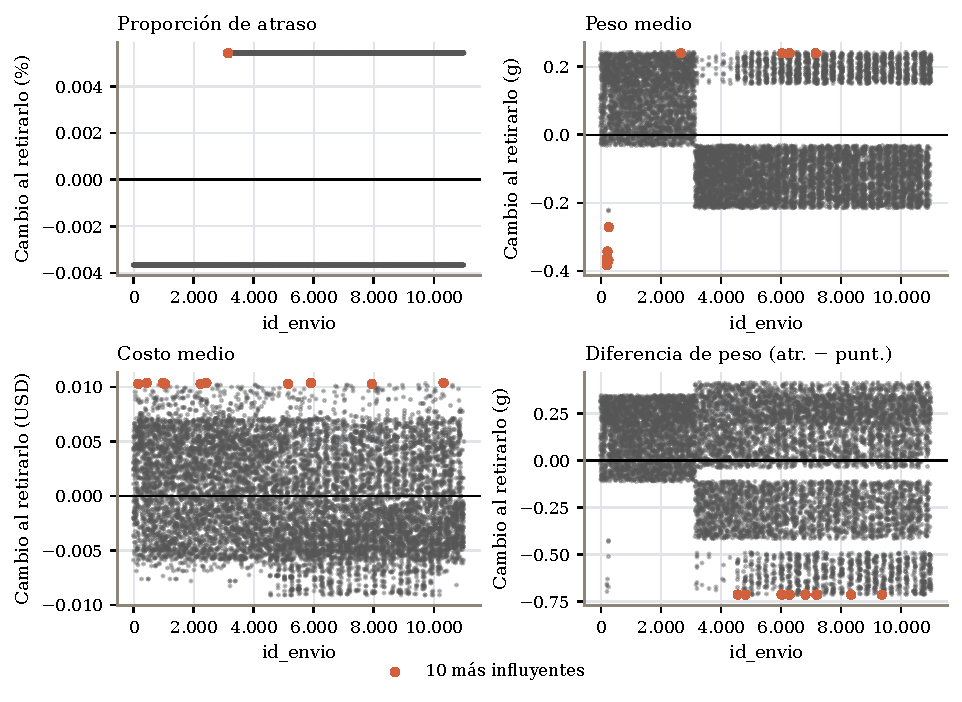
\includegraphics[width=\linewidth,height=0.42\textheight,keepaspectratio]{../../outputs/validacion_completa/figuras/fig_jk_1_influencia.pdf}\caption{Influencia de cada envío en los resultados principales (\emph{jackknife}).}\label{fig:E1}\end{figure}

\textbf{Escenarios.} Las reglas se fijaron antes de calcular, con umbrales obtenidos de los datos completos (tabla \ref{tab:E2}). El CSV original no se modifica: cada escenario es una vista. Los escenarios restringidos describen subpoblaciones y no estiman el mismo parámetro.

{\scriptsize\setlength{\tabcolsep}{3pt}
\begin{longtable}{@{}l l r r l@{}}
\caption{Reglas, umbrales y tamaños de los escenarios de sensibilidad.}\label{tab:E2}\\\toprule
Escenario & Variable & Inferior & Superior & Regla\\\midrule\endfirsthead
\multicolumn{5}{@{}l}{\emph{Continuación de la tabla \ref{tab:E2}}}\\\toprule
Escenario & Variable & Inferior & Superior & Regla\\\midrule\endhead
\bottomrule\endfoot
Winsor. 1/99 & Peso & 1.030,0 & 5.964,0 & cuantiles 0.01/0.99; interpolación lineal\\
Winsor. 1/99 & Costo & 108,00 & 304,00 & cuantiles 0.01/0.99; interpolación lineal\\
Excl. IQR & Llamadas & 0 & 8,0000 & fuera de [Q1$-$1.5 IQR, Q3+1.5 IQR]; unión entre variables\\
Excl. IQR & Costo & 46,00 & 374,00 & fuera de [Q1$-$1.5 IQR, Q3+1.5 IQR]; unión entre variables\\
Excl. IQR & Compras previas & 1,5000 & 5,5000 & fuera de [Q1$-$1.5 IQR, Q3+1.5 IQR]; unión entre variables\\
Excl. IQR & Descuento & $-$5,0000 & 19,00 & fuera de [Q1$-$1.5 IQR, Q3+1.5 IQR]; unión entre variables\\
Excl. IQR & Peso & $-$2.976,2 & 9.865,8 & fuera de [Q1$-$1.5 IQR, Q3+1.5 IQR]; unión entre variables\\
Desc. $\le$ 10 & Descuento & --- & 10,00 & retener descuento $\le$10\\
\midrule\multicolumn{5}{@{}l}{\emph{Tamaño de cada escenario}}\\
Completos & retenidos 10.999 & excluidos 0 & modificados 0 & tasa de atraso 0,5967\\
Winsor. 1/99 & retenidos 10.999 & excluidos 0 & modificados 425 & tasa de atraso 0,5967\\
Excl. IQR & retenidos 7.971 & excluidos 3.028 & modificados 0 & tasa de atraso 0,4952\\
Desc. $\le$ 10 & retenidos 8.352 & excluidos 2.647 & modificados 0 & tasa de atraso 0,4689\\
\end{longtable}}

{\scriptsize\setlength{\tabcolsep}{3pt}
\begin{longtable}{@{}l l r r r r@{}}
\caption{Efecto y $p$ de permutación ajustado por Holm de las siete pruebas en cada escenario.}\label{tab:E3}\\\toprule
ID & Contraste & Completos & Winsor. 1/99 & Excl. IQR & Desc. $\le$ 10\\\midrule\endfirsthead
\multicolumn{6}{@{}l}{\emph{Continuación de la tabla \ref{tab:E3}}}\\\toprule
ID & Contraste & Completos & Winsor. 1/99 & Excl. IQR & Desc. $\le$ 10\\\midrule\endhead
\bottomrule\endfoot
T01 & Modalidad & 0,0082 (0,6911) & 0,0082 (0,6816) & 0,0134 (0,7147) & 0,0049 (1,0000)\\
T02 & Peso & $-$896,03 (0,0007)* & $-$897,37 (0,0007)* & $-$449,62 (0,0007)* & $-$283,75 (0,0007)*\\
T03 & Descuento & 13,12 (0,0007)* & 13,12 (0,0007)* & 0,8579 (0,0007)* & $-$0,0825 (0,7835)\\
E1 & Peso (rangos) & $-$0,3130 (0,0007)* & $-$0,3131 (0,0007)* & $-$0,1589 (0,0007)* & $-$0,1015 (0,0007)*\\
E2 & Importancia alta & 0,0581 (0,0016)* & 0,0581 (0,0012)* & 0,0469 (0,0858) & 0,0443 (0,1435)\\
E3 & Descuento $>$ 10 & 0,5311 (0,0007)* & 0,5311 (0,0007)* & 0,5322 (0,0007)* & no evaluable\\
E4 & Costo & $-$7,2095 (0,0007)* & $-$7,1916 (0,0007)* & $-$0,9895 (0,7147) & 0,2889 (1,0000)\\
\end{longtable}}
{\footnotesize * Se rechaza $H_0$ al 5\,\% con Holm sobre la familia completa del escenario. E3 no es evaluable con descuento $\le 10$: el escenario suprime uno de sus grupos.\par}\medskip

{\tiny\setlength{\tabcolsep}{3pt}
\begin{longtable}{@{}l l l l l l@{}}
\caption{Correlaciones y asociaciones de S1 por escenario: estimación e IC \emph{bootstrap} 95\,\%.}\label{tab:E4}\\\toprule
ID & Par & Completos & Winsor. 1/99 & Excl. IQR & Desc. $\le$ 10\\\midrule\endfirsthead
\multicolumn{6}{@{}l}{\emph{Continuación de la tabla \ref{tab:E4}}}\\\toprule
ID & Par & Completos & Winsor. 1/99 & Excl. IQR & Desc. $\le$ 10\\\midrule\endhead
\bottomrule\endfoot
COR-011 & Compras previas -- Atraso & $-$0,056 [$-$0,075; $-$0,037] & $-$0,056 [$-$0,074; $-$0,036] & $-$0,042 [$-$0,063; $-$0,019] & $-$0,012 [$-$0,034; 0,010]\,\dag\\
COR-012 & Costo -- Atraso & $-$0,074 [$-$0,092; $-$0,055] & $-$0,074 [$-$0,092; $-$0,055] & $-$0,010 [$-$0,033; 0,011]\,\dag & 0,003 [$-$0,018; 0,024]\,\dag\\
COR-013 & Descuento -- Atraso & 0,397 [0,388; 0,407] & 0,397 [0,388; 0,406] & 0,121 [0,100; 0,142] & $-$0,014 [$-$0,036; 0,007]\,\dag\\
COR-014 & Llamadas -- Atraso & $-$0,067 [$-$0,086; $-$0,048] & $-$0,067 [$-$0,086; $-$0,048] & $-$0,017 [$-$0,039; 0,005]\,\dag & 0,004 [$-$0,018; 0,025]\,\dag\\
COR-015 & Peso -- Atraso & $-$0,269 [$-$0,287; $-$0,251] & $-$0,270 [$-$0,287; $-$0,251] & $-$0,139 [$-$0,161; $-$0,117] & $-$0,088 [$-$0,109; $-$0,067]\\
COR-016 & Compras previas -- Costo & 0,194 [0,176; 0,212] & 0,194 [0,176; 0,211] & 0,267 [0,246; 0,287] & 0,228 [0,208; 0,248]\\
COR-017 & Compras previas -- Descuento & $-$0,094 [$-$0,112; $-$0,075] & $-$0,094 [$-$0,112; $-$0,075] & $-$0,020 [$-$0,042; 0,001]\,\dag & 0,015 [$-$0,007; 0,037]\,\dag\\
COR-018 & Compras previas -- Atraso & $-$0,075 [$-$0,094; $-$0,056] & $-$0,075 [$-$0,093; $-$0,055] & $-$0,040 [$-$0,061; $-$0,018] & $-$0,014 [$-$0,036; 0,008]\,\dag\\
COR-019 & Compras previas -- Llamadas & 0,273 [0,256; 0,290] & 0,273 [0,256; 0,290] & 0,354 [0,335; 0,372] & 0,291 [0,272; 0,310]\\
COR-020 & Compras previas -- Peso & $-$0,235 [$-$0,253; $-$0,216] & $-$0,235 [$-$0,253; $-$0,216] & $-$0,385 [$-$0,405; $-$0,364] & $-$0,341 [$-$0,360; $-$0,322]\\
COR-021 & Costo -- Descuento & $-$0,116 [$-$0,134; $-$0,098] & $-$0,116 [$-$0,134; $-$0,098] & $-$0,016 [$-$0,038; 0,006]\,\dag & 0,008 [$-$0,013; 0,030]\,\dag\\
COR-022 & Costo -- Atraso & $-$0,072 [$-$0,090; $-$0,053] & $-$0,072 [$-$0,090; $-$0,053] & $-$0,008 [$-$0,031; 0,014]\,\dag & 0,005 [$-$0,016; 0,027]\,\dag\\
COR-023 & Costo -- Llamadas & 0,294 [0,275; 0,312] & 0,294 [0,275; 0,312] & 0,346 [0,324; 0,367] & 0,339 [0,318; 0,360]\\
COR-024 & Costo -- Peso & $-$0,132 [$-$0,152; $-$0,112] & $-$0,132 [$-$0,152; $-$0,112] & $-$0,295 [$-$0,316; $-$0,273] & $-$0,325 [$-$0,345; $-$0,305]\\
COR-025 & Descuento -- Atraso & 0,335 [0,319; 0,351] & 0,335 [0,319; 0,351] & 0,070 [0,048; 0,093] & $-$0,014 [$-$0,036; 0,007]\,\dag\\
COR-026 & Descuento -- Llamadas & $-$0,104 [$-$0,123; $-$0,085] & $-$0,104 [$-$0,122; $-$0,086] & $-$0,025 [$-$0,047; $-$0,003] & 0,004 [$-$0,017; 0,025]\,\dag\\
COR-027 & Descuento -- Peso & $-$0,316 [$-$0,333; $-$0,298] & $-$0,316 [$-$0,333; $-$0,299] & $-$0,081 [$-$0,103; $-$0,059] & 0,007 [$-$0,015; 0,029]\,\dag\\
COR-028 & Llamadas -- Atraso & $-$0,064 [$-$0,083; $-$0,046] & $-$0,064 [$-$0,083; $-$0,046] & $-$0,017 [$-$0,039; 0,005]\,\dag & 0,002 [$-$0,019; 0,023]\,\dag\\
COR-029 & Llamadas -- Peso & $-$0,233 [$-$0,252; $-$0,214] & $-$0,233 [$-$0,251; $-$0,214] & $-$0,330 [$-$0,351; $-$0,309] & $-$0,347 [$-$0,367; $-$0,327]\\
COR-030 & Peso -- Atraso & $-$0,266 [$-$0,284; $-$0,248] & $-$0,266 [$-$0,284; $-$0,248] & $-$0,138 [$-$0,159; $-$0,116] & $-$0,088 [$-$0,109; $-$0,067]\\
ASO-001 & Bodega -- Calificación & 0,015 [0,017; 0,032] & 0,015 [0,017; 0,032] & 0,021 [0,021; 0,040] & 0,022 [0,021; 0,040]\\
ASO-002 & Bodega -- Atraso & 0,010 [0,008; 0,036] & 0,010 [0,008; 0,036] & 0,024 [0,013; 0,051] & 0,011 [0,008; 0,040]\\
ASO-003 & Bodega -- Género & 0,009 [0,008; 0,034] & 0,009 [0,007; 0,035] & 0,020 [0,012; 0,048] & 0,018 [0,010; 0,046]\\
ASO-004 & Bodega -- Importancia & 0,019 [0,016; 0,038] & 0,019 [0,015; 0,038] & 0,017 [0,015; 0,041] & 0,018 [0,016; 0,041]\\
ASO-005 & Bodega -- Modalidad & 0,001 [0,010; 0,028] & 0,001 [0,010; 0,028] & 0,006 [0,012; 0,034] & 0,005 [0,012; 0,033]\\
ASO-006 & Calificación -- Atraso & 0,017 [0,009; 0,041] & 0,017 [0,010; 0,040] & 0,029 [0,016; 0,055] & 0,027 [0,015; 0,053]\\
ASO-007 & Calificación -- Género & 0,016 [0,009; 0,041] & 0,016 [0,009; 0,040] & 0,022 [0,012; 0,050] & 0,021 [0,012; 0,048]\\
ASO-008 & Calificación -- Importancia & 0,018 [0,015; 0,037] & 0,018 [0,015; 0,037] & 0,024 [0,019; 0,046] & 0,029 [0,022; 0,049]\\
ASO-009 & Calificación -- Modalidad & 0,017 [0,015; 0,036] & 0,017 [0,014; 0,037] & 0,028 [0,022; 0,049] & 0,024 [0,019; 0,045]\\
ASO-010 & Género -- Atraso & 0,005 [0,000; 0,024] & 0,005 [0,000; 0,024] & 0,014 [0,001; 0,036] & 0,013 [0,001; 0,034]\\
ASO-011 & Género -- Importancia & 0,010 [0,003; 0,031] & 0,010 [0,003; 0,031] & 0,008 [0,003; 0,033] & 0,009 [0,003; 0,034]\\
ASO-012 & Género -- Modalidad & 0,018 [0,005; 0,039] & 0,018 [0,005; 0,038] & 0,019 [0,005; 0,044] & 0,009 [0,003; 0,034]\\
ASO-013 & Importancia -- Atraso & 0,033 [0,017; 0,053] & 0,033 [0,017; 0,053] & 0,027 [0,009; 0,051] & 0,026 [0,010; 0,049]\\
ASO-014 & Importancia -- Modalidad & 0,010 [0,006; 0,028] & 0,010 [0,006; 0,028] & 0,012 [0,007; 0,032] & 0,014 [0,008; 0,034]\\
ASO-015 & Modalidad -- Atraso & 0,008 [0,003; 0,029] & 0,008 [0,003; 0,030] & 0,013 [0,004; 0,038] & 0,005 [0,003; 0,031]\\
\end{longtable}}
{\footnotesize \dag\ Cambia el signo o la inclusión del cero respecto de los datos completos.\par}\medskip

{\tiny\setlength{\tabcolsep}{3pt}
\begin{longtable}{@{}l >{\raggedright\arraybackslash}p{3.0cm} >{\raggedright\arraybackslash}p{3.2cm} r r r r@{}}
\caption{Los 128 estimandos de la tabla A-1 en cada escenario.}\label{tab:E5}\\\toprule
ID & Estimando & Grupo & Completos & Winsor. 1/99 & Excl. IQR & Desc. $\le$ 10\\\midrule\endfirsthead
\multicolumn{7}{@{}l}{\emph{Continuación de la tabla \ref{tab:E5}}}\\\toprule
ID & Estimando & Grupo & Completos & Winsor. 1/99 & Excl. IQR & Desc. $\le$ 10\\\midrule\endhead
\bottomrule\endfoot
PAR-001 & Media, costo & global & 210,20 & 210,23 & 213,69 & 214,63\\
PAR-002 & Media, llamadas & global & 4,0545 & 4,0545 & 4,1330 & 4,1517\\
PAR-003 & Media, peso & global & 3.634,0 & 3.633,2 & 3.956,7 & 4.035,6\\
PAR-004 & Proporción, atraso & 1 & 0,5967 & 0,5967 & 0,4952 & 0,4689\\
EFE-001 & $d_{av}$, compras previas & atras. $-$ punt. & $-$0,1133 & $-$0,1133 & $-$0,0834 & $-$0,0235\\
EFE-002 & $d_{av}$, costo & atras. $-$ punt. & $-$0,1505 & $-$0,1508 & $-$0,0205 & 0,0060\\
EFE-003 & $d_{av}$, descuento & atras. $-$ punt. & 0,9600 & 0,9600 & 0,2432 & $-$0,0286\\
EFE-004 & $d_{av}$, llamadas & atras. $-$ punt. & $-$0,1367 & $-$0,1367 & $-$0,0332 & 0,0074\\
EFE-005 & $d_{av}$, peso & atras. $-$ punt. & $-$0,5689 & $-$0,5705 & $-$0,2803 & $-$0,1770\\
EFE-006 & Dif. de medias, costo & atras. $-$ punt. & $-$7,2095 & $-$7,1916 & $-$0,9895 & 0,2889\\
EFE-007 & Dif. de medias, descuento & atras. $-$ punt. & 13,12 & 13,12 & 0,8579 & $-$0,0825\\
EFE-008 & Dif. de medias, peso & atras. $-$ punt. & $-$896,03 & $-$897,37 & $-$449,62 & $-$283,75\\
EFE-009 & Dif. de proporciones, descuento & Descuento $>$ 10 - Descuento $\le$ 10 & 0,5311 & 0,5311 & 0,5322 & no evaluable\\
EFE-010 & Dif. de proporciones, importancia & Importancia=alta - Importancia en \{baja, media\} & 0,0581 & 0,0581 & 0,0469 & 0,0443\\
EFE-011 & Biserial de rangos, peso & atras. $-$ punt. & $-$0,3130 & $-$0,3131 & $-$0,1589 & $-$0,1015\\
EFE-012 & Riesgo relativo, descuento & Descuento $>$ 10 / Descuento $\le$ 10 & 2,1328 & 2,1328 & 2,1377 & no evaluable\\
EFE-013 & Riesgo relativo, importancia & Importancia=alta / Importancia en \{baja, media\} & 1,0982 & 1,0982 & 1,0954 & 1,0953\\
DES-001 & Asimetría, compras previas & global & 1,6819 & 1,6819 & 0,3115 & 1,5405\\
DES-002 & Asimetría, costo & global & $-$0,1571 & $-$0,1497 & $-$0,2059 & $-$0,2515\\
DES-003 & Asimetría, descuento & global & 1,7989 & 1,7989 & 0,7935 & 0,0032\\
DES-004 & Asimetría, llamadas & global & 0,3919 & 0,3919 & 0,3834 & 0,3623\\
DES-005 & Asimetría, peso & global & $-$0,2497 & $-$0,2548 & $-$0,6352 & $-$0,7448\\
DES-006 & Curtosis (exceso), compras previas & global & 4,0063 & 4,0063 & $-$0,9336 & 3,6031\\
DES-007 & Curtosis (exceso), costo & global & $-$0,9722 & $-$1,0163 & $-$0,9357 & $-$0,9025\\
DES-008 & Curtosis (exceso), descuento & global & 2,0006 & 2,0006 & 1,0380 & $-$1,2325\\
DES-009 & Curtosis (exceso), llamadas & global & $-$0,3090 & $-$0,3090 & $-$0,3886 & $-$0,4036\\
DES-010 & Curtosis (exceso), peso & global & $-$1,4477 & $-$1,4584 & $-$1,1289 & $-$0,9750\\
DES-011 & DE, compras previas & global & 1,5229 & 1,5229 & 0,9913 & 1,5129\\
DES-012 & DE, costo & atrasada & 48,05 & 47,88 & 48,47 & 48,27\\
DES-013 & DE, costo & global & 48,06 & 47,86 & 48,23 & 47,99\\
DES-014 & DE, costo & puntual & 47,76 & 47,52 & 48,00 & 47,76\\
DES-015 & DE, descuento & atrasada & 19,11 & 19,11 & 4,0810 & 2,8873\\
DES-016 & DE, descuento & global & 16,21 & 16,21 & 3,5476 & 2,8823\\
DES-017 & DE, descuento & puntual & 2,8777 & 2,8777 & 2,8695 & 2,8777\\
DES-018 & DE, llamadas & global & 1,1415 & 1,1415 & 1,1776 & 1,1674\\
DES-019 & DE, peso & atrasada & 1.576,1 & 1.572,6 & 1.636,5 & 1.632,3\\
DES-020 & DE, peso & global & 1.635,4 & 1.633,3 & 1.619,4 & 1.607,7\\
DES-021 & DE, peso & puntual & 1.574,0 & 1.573,4 & 1.571,1 & 1.574,0\\
DES-022 & IQR, compras previas & global & 1,0000 & 1,0000 & 1,0000 & 1,0000\\
DES-023 & IQR, costo & global & 82,00 & 82,00 & 81,00 & 80,00\\
DES-024 & IQR, descuento & global & 6,0000 & 6,0000 & 5,0000 & 5,0000\\
DES-025 & IQR, llamadas & global & 2,0000 & 2,0000 & 2,0000 & 2,0000\\
DES-026 & IQR, peso & global & 3.210,5 & 3.210,5 & 3.288,5 & 3.299,2\\
DES-027 & Máximo, compras previas & global & 10,00 & 10,00 & 5,0000 & 10,00\\
DES-028 & Máximo, costo & global & 310,00 & 304,00 & 310,00 & 310,00\\
DES-029 & Máximo, descuento & global & 65,00 & 65,00 & 19,00 & 10,00\\
DES-030 & Máximo, llamadas & global & 7,0000 & 7,0000 & 7,0000 & 7,0000\\
DES-031 & Máximo, peso & global & 7.846,0 & 5.964,0 & 6.102,0 & 6.102,0\\
DES-032 & Media, compras previas & atrasada & 3,4981 & 3,4981 & 3,2404 & 3,6348\\
DES-033 & Media, compras previas & global & 3,5676 & 3,5676 & 3,2821 & 3,6537\\
DES-034 & Media, compras previas & puntual & 3,6704 & 3,6704 & 3,3231 & 3,6704\\
DES-035 & Media, costo & atrasada & 207,29 & 207,33 & 213,19 & 214,79\\
DES-036 & Media, costo & puntual & 214,50 & 214,52 & 214,18 & 214,50\\
DES-037 & Media, descuento & atrasada & 18,66 & 18,66 & 6,4201 & 5,4635\\
DES-038 & Media, descuento & global & 13,37 & 13,37 & 5,9870 & 5,5073\\
DES-039 & Media, descuento & puntual & 5,5460 & 5,5460 & 5,5621 & 5,5460\\
DES-040 & Media, llamadas & atrasada & 3,9915 & 3,9915 & 4,1133 & 4,1563\\
DES-041 & Media, llamadas & puntual & 4,1477 & 4,1477 & 4,1523 & 4,1477\\
DES-042 & Media, peso & atrasada & 3.272,6 & 3.271,3 & 3.729,7 & 3.884,9\\
DES-043 & Media, peso & puntual & 4.168,7 & 4.168,6 & 4.179,3 & 4.168,7\\
DES-044 & Mediana, compras previas & atrasada & 3,0000 & 3,0000 & 3,0000 & 3,0000\\
DES-045 & Mediana, compras previas & global & 3,0000 & 3,0000 & 3,0000 & 3,0000\\
DES-046 & Mediana, compras previas & puntual & 3,0000 & 3,0000 & 3,0000 & 3,0000\\
DES-047 & Mediana, costo & atrasada & 209,00 & 209,00 & 219,00 & 222,00\\
DES-048 & Mediana, costo & global & 214,00 & 214,00 & 220,00 & 222,00\\
DES-049 & Mediana, costo & puntual & 222,00 & 222,00 & 221,00 & 222,00\\
DES-050 & Mediana, descuento & atrasada & 9,0000 & 9,0000 & 6,0000 & 5,0000\\
DES-051 & Mediana, descuento & global & 7,0000 & 7,0000 & 6,0000 & 6,0000\\
DES-052 & Mediana, descuento & puntual & 6,0000 & 6,0000 & 6,0000 & 6,0000\\
DES-053 & Mediana, llamadas & atrasada & 4,0000 & 4,0000 & 4,0000 & 4,0000\\
DES-054 & Mediana, llamadas & global & 4,0000 & 4,0000 & 4,0000 & 4,0000\\
DES-055 & Mediana, llamadas & puntual & 4,0000 & 4,0000 & 4,0000 & 4,0000\\
DES-056 & Mediana, peso & atrasada & 3.231,0 & 3.231,0 & 4.278,0 & 4.435,0\\
DES-057 & Mediana, peso & global & 4.149,0 & 4.149,0 & 4.520,0 & 4.581,0\\
DES-058 & Mediana, peso & puntual & 4.674,0 & 4.674,0 & 4.687,5 & 4.674,0\\
DES-059 & Mínimo, compras previas & global & 2,0000 & 2,0000 & 2,0000 & 2,0000\\
DES-060 & Mínimo, costo & global & 96,00 & 108,00 & 96,00 & 96,00\\
DES-061 & Mínimo, descuento & global & 1,0000 & 1,0000 & 1,0000 & 1,0000\\
DES-062 & Mínimo, llamadas & global & 2,0000 & 2,0000 & 2,0000 & 2,0000\\
DES-063 & Mínimo, peso & global & 1.001,0 & 1.030,0 & 1.001,0 & 1.001,0\\
DES-064 & Extremos IQR (\%), costo & global & 0 & 0 & 0 & 0\\
DES-065 & Extremos IQR (\%), llamadas & global & 0 & 0 & 0 & 0\\
DES-066 & Extremos IQR (\%), peso & global & 0 & 0 & 0 & 0\\
DES-067 & \% suma top 1\%, costo & global & 1,4485 & 1,4330 & 1,4291 & 1,4261\\
DES-068 & \% suma top 1\%, llamadas & global & 1,7110 & 1,7110 & 1,6786 & 1,6756\\
DES-069 & \% suma top 1\%, peso & global & 1,6538 & 1,6268 & 1,4995 & 1,4742\\
DES-070 & Proporción, bodega & A & 0,1667 & 0,1667 & 0,1695 & 0,1676\\
DES-071 & Proporción, bodega & B & 0,1667 & 0,1667 & 0,1660 & 0,1669\\
DES-072 & Proporción, bodega & C & 0,1667 & 0,1667 & 0,1669 & 0,1662\\
DES-073 & Proporción, bodega & D & 0,1667 & 0,1667 & 0,1684 & 0,1671\\
DES-074 & Proporción, bodega & F & 0,3333 & 0,3333 & 0,3293 & 0,3321\\
DES-075 & Proporción, calificación & 1 & 0,2032 & 0,2032 & 0,2036 & 0,2039\\
DES-076 & Proporción, calificación & 2 & 0,1968 & 0,1968 & 0,1936 & 0,1941\\
DES-077 & Proporción, calificación & 3 & 0,2036 & 0,2036 & 0,2059 & 0,2063\\
DES-078 & Proporción, calificación & 4 & 0,1990 & 0,1990 & 0,1995 & 0,2000\\
DES-079 & Proporción, calificación & 5 & 0,1974 & 0,1974 & 0,1975 & 0,1958\\
DES-080 & Proporción, atraso & 0 & 0,4033 & 0,4033 & 0,5048 & 0,5311\\
DES-081 & Proporción, género & F & 0,5041 & 0,5041 & 0,5012 & 0,5011\\
DES-082 & Proporción, género & M & 0,4959 & 0,4959 & 0,4988 & 0,4989\\
DES-083 & Proporción, importancia & high & 0,0862 & 0,0862 & 0,0767 & 0,0811\\
DES-084 & Proporción, importancia & low & 0,4816 & 0,4816 & 0,4960 & 0,4877\\
DES-085 & Proporción, importancia & medium & 0,4322 & 0,4322 & 0,4273 & 0,4313\\
DES-086 & Proporción, modalidad & Flight & 0,1616 & 0,1616 & 0,1641 & 0,1609\\
DES-087 & Proporción, modalidad & Road & 0,1600 & 0,1600 & 0,1576 & 0,1621\\
DES-088 & Proporción, modalidad & Ship & 0,6784 & 0,6784 & 0,6783 & 0,6770\\
DES-089 & Q1, compras previas & global & 3,0000 & 3,0000 & 3,0000 & 3,0000\\
DES-090 & Q1, costo & global & 169,00 & 169,00 & 173,00 & 174,00\\
DES-091 & Q1, descuento & global & 4,0000 & 4,0000 & 3,0000 & 3,0000\\
DES-092 & Q1, llamadas & global & 3,0000 & 3,0000 & 3,0000 & 3,0000\\
DES-093 & Q1, peso & global & 1.839,5 & 1.839,5 & 1.955,5 & 1.981,8\\
DES-094 & Q3, compras previas & global & 4,0000 & 4,0000 & 4,0000 & 4,0000\\
DES-095 & Q3, costo & global & 251,00 & 251,00 & 254,00 & 254,00\\
DES-096 & Q3, descuento & global & 10,00 & 10,00 & 8,0000 & 8,0000\\
DES-097 & Q3, llamadas & global & 5,0000 & 5,0000 & 5,0000 & 5,0000\\
DES-098 & Q3, peso & global & 5.050,0 & 5.050,0 & 5.244,0 & 5.281,0\\
DES-099 & Tasa de atraso, bodega & Bodega=A & 0,5865 & 0,5865 & 0,4819 & 0,4586\\
DES-100 & Tasa de atraso, bodega & Bodega=B & 0,6023 & 0,6023 & 0,5110 & 0,4770\\
DES-101 & Tasa de atraso, calificación & Calificación=1 & 0,5875 & 0,5875 & 0,4806 & 0,4586\\
DES-102 & Tasa de atraso, calificación & Calificación=5 & 0,6066 & 0,6066 & 0,5032 & 0,4777\\
DES-103 & Tasa de atraso, descuento & Descuento $\le$ 10 & 0,4689 & 0,4689 & 0,4678 & no evaluable\\
DES-104 & Tasa de atraso, descuento & Descuento $>$ 10 & 1,0000 & 1,0000 & 1,0000 & no evaluable\\
DES-105 & Tasa de atraso, género & Género=Fem. & 0,5944 & 0,5944 & 0,4881 & 0,4626\\
DES-106 & Tasa de atraso, género & Género=Masc. & 0,5990 & 0,5990 & 0,5023 & 0,4752\\
DES-107 & Tasa de atraso, importancia & Importancia en \{baja, media\} & 0,5917 & 0,5917 & 0,4916 & 0,4653\\
DES-108 & Tasa de atraso, importancia & Importancia=alta & 0,6498 & 0,6498 & 0,5385 & 0,5096\\
DES-109 & Tasa de atraso, importancia & Importancia=media & 0,5905 & 0,5905 & 0,4865 & 0,4595\\
DES-110 & Tasa de atraso, modalidad & Modalidad=Avión & 0,6016 & 0,6016 & 0,5069 & 0,4732\\
DES-111 & Tasa de atraso, modalidad & Modalidad=Carretera & 0,5881 & 0,5881 & 0,4833 & 0,4645\\
\end{longtable}}
{\footnotesize Los IC percentil y BCa por escenario están en \texttt{sensibilidad\_parametros.csv}. ``No evaluable'': el escenario elimina el grupo o deja la variable sin variación.\par}\medskip

\begin{figure}[H]\centering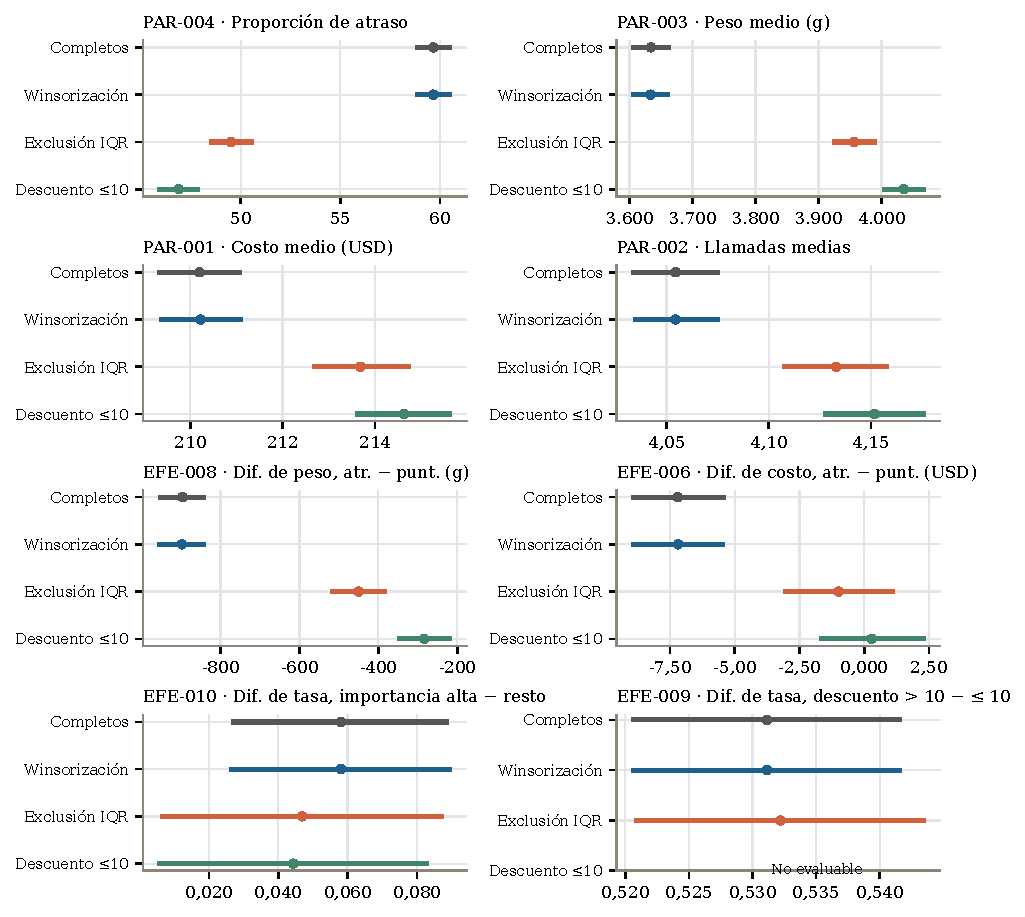
\includegraphics[width=\linewidth,height=0.55\textheight,keepaspectratio]{../../outputs/validacion_completa/figuras/fig_sens_parametros.pdf}\caption{Cambio relativo de los parámetros y efectos por escenario.}\label{fig:E2}\end{figure}

\begin{figure}[H]\centering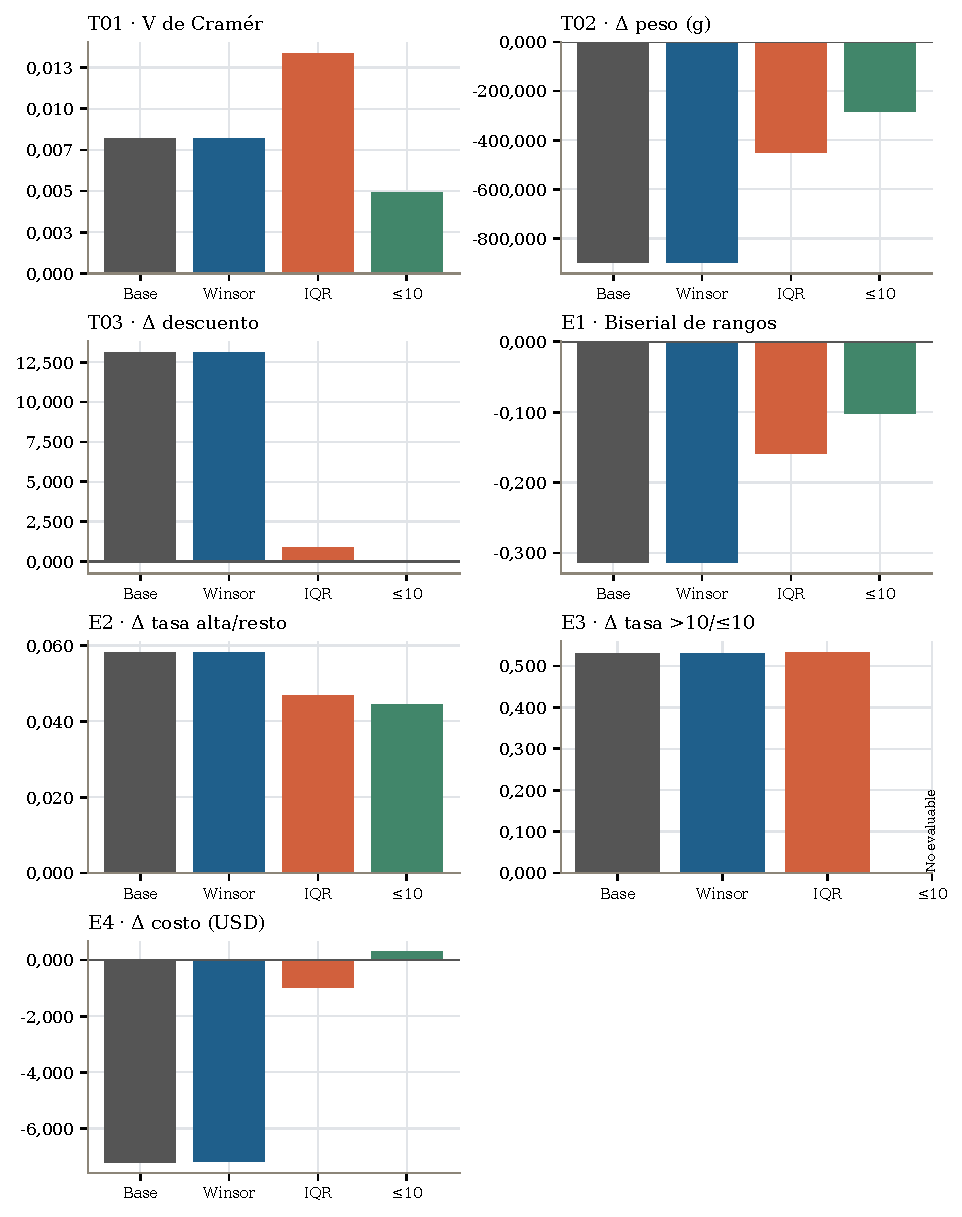
\includegraphics[width=\linewidth,height=0.55\textheight,keepaspectratio]{../../outputs/validacion_completa/figuras/fig_sens_efectos_pruebas.pdf}\caption{Efectos de las siete pruebas por escenario.}\label{fig:E3}\end{figure}

\begin{figure}[H]\centering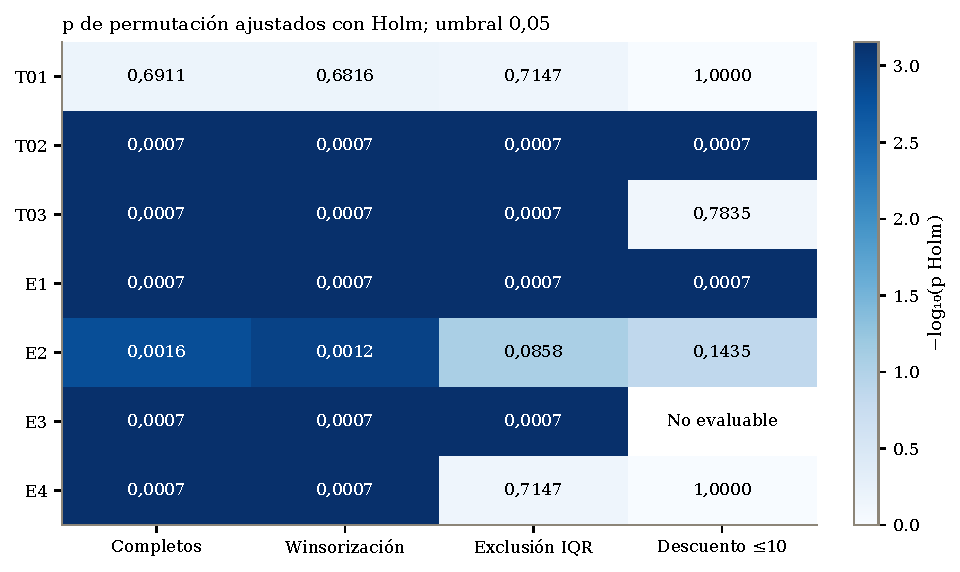
\includegraphics[width=\linewidth,height=0.55\textheight,keepaspectratio]{../../outputs/validacion_completa/figuras/fig_sens_holm_escenarios.pdf}\caption{Decisiones con Holm por escenario.}\label{fig:E4}\end{figure}

\begin{figure}[H]\centering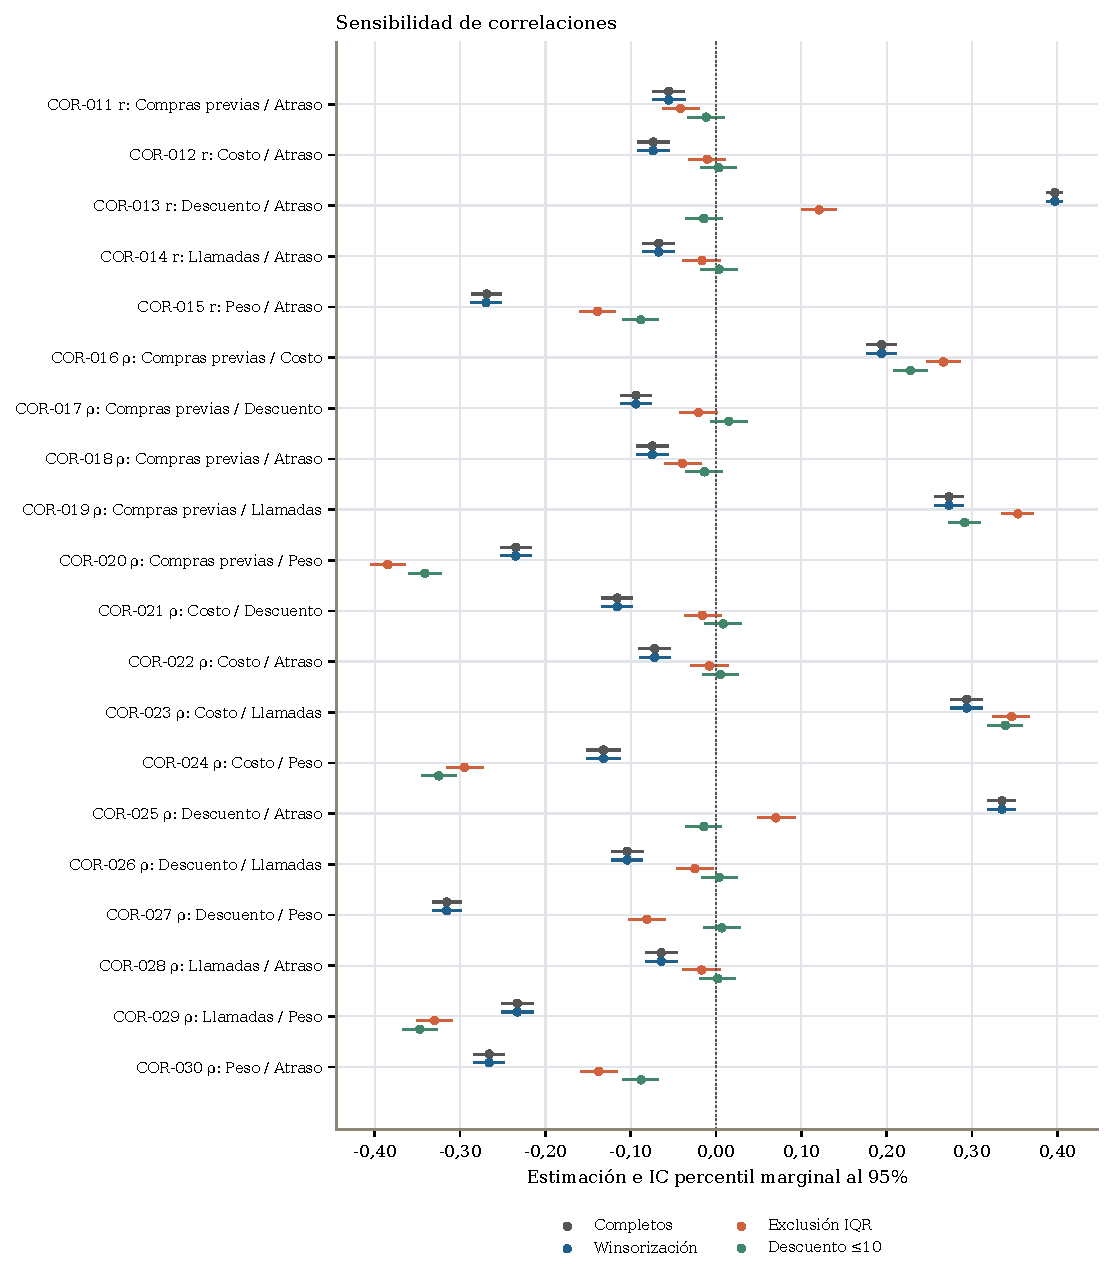
\includegraphics[width=\linewidth,height=0.55\textheight,keepaspectratio]{../../outputs/validacion_completa/figuras/fig_sens_correlaciones_intervalos.pdf}\caption{IC de las 20 correlaciones por escenario.}\label{fig:E5}\end{figure}

\begin{figure}[H]\centering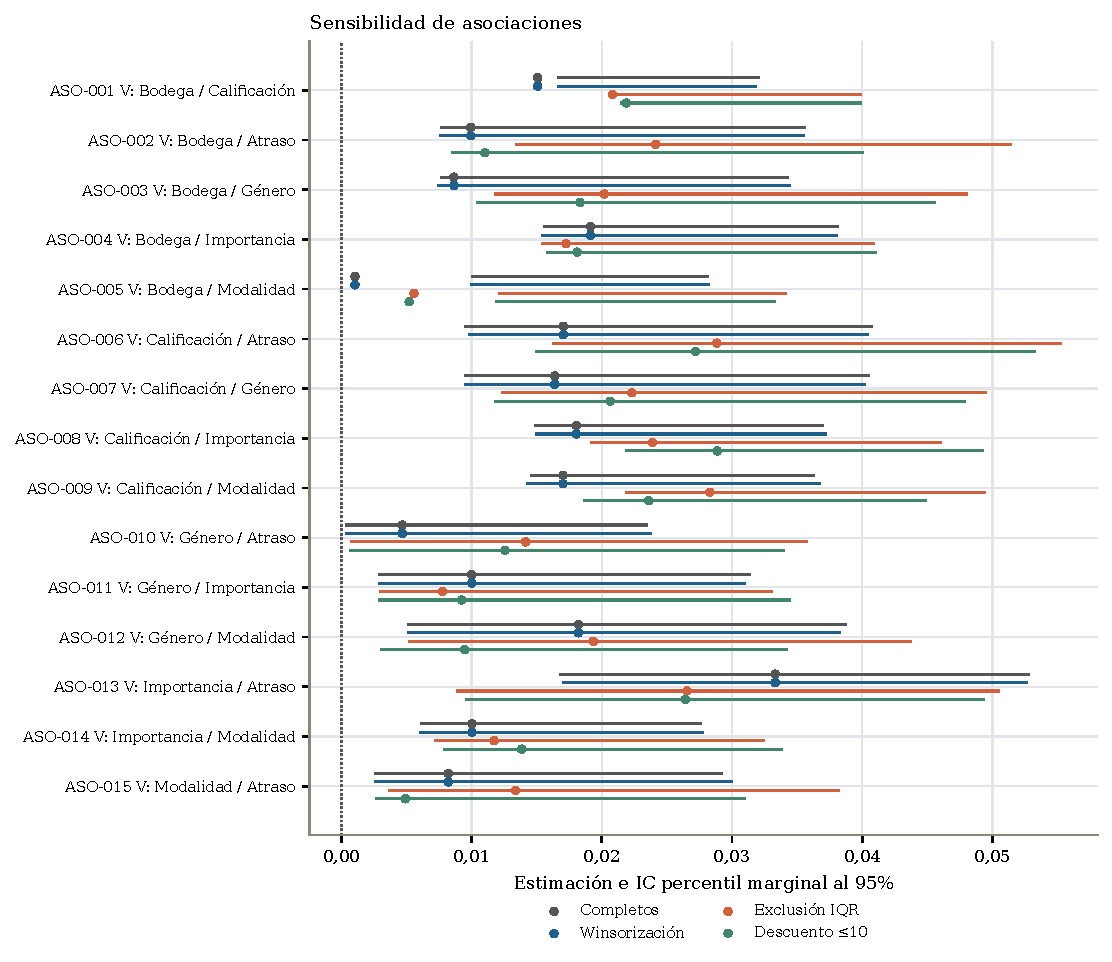
\includegraphics[width=\linewidth,height=0.55\textheight,keepaspectratio]{../../outputs/validacion_completa/figuras/fig_sens_asociaciones_intervalos.pdf}\caption{IC de las 15 asociaciones por escenario.}\label{fig:E6}\end{figure}

\clearpage\section{Anexo F. Matriz de resultados validados para S3}\label{anx:F}

\setcounter{table}{0}\setcounter{figure}{0}\renewcommand{\thetable}{F-\arabic{table}}\renewcommand{\thefigure}{F-\arabic{figure}}

La tabla \ref{tab:F1} reproduce \texttt{outputs/resultados\_validados.csv}, archivo de entrada a S3, con el estado y la recomendación de cada resultado discutido en el cuerpo. La tabla \ref{tab:F2} comprueba la cobertura del 100\,\% del inventario: cada uno de los 194 resultados de S1 tiene una validación o una excepción metodológica explícita.

{\scriptsize\setlength{\tabcolsep}{3pt}
\begin{longtable}{@{}l >{\raggedright\arraybackslash}p{4.2cm} >{\raggedright\arraybackslash}p{2.3cm} >{\raggedright\arraybackslash}p{6.4cm}@{}}
\caption{Resultados validados, estado y recomendación para S3.}\label{tab:F1}\\\toprule
ID & Resultado & Estado & Recomendación para S3\\\midrule\endfirsthead
\multicolumn{4}{@{}l}{\emph{Continuación de la tabla \ref{tab:F1}}}\\\toprule
ID & Resultado & Estado & Recomendación para S3\\\midrule\endhead
\bottomrule\endfoot
PAR-1 & Proporción de atraso & respaldado & Usar 59,67 \% [58,75; 60,58] como tasa de referencia; reportar por segmento de descuento.\\
PAR-2 & Peso medio & respaldado & Media válida como resumen, pero el peso es bimodal: modelar con tramos o términos no lineales.\\
PAR-3 & Costo medio & respaldado & Variable de bajo poder explicativo para el atraso; conservar solo como control.\\
PAR-4 & Llamadas medias & respaldado & Media estable; las llamadas pueden ser posteriores al envío: revisar su temporalidad antes de usarlas como predictor.\\
EFE-1 & Diferencia de peso medio (atrasado $-$ puntual) & respaldado, magnitud sensible & Incluir el peso en S3; su efecto se reduce fuera del descuento alto: estimar interacción peso $\times$ segmento.\\
T01 & Prueba $\chi^2$ de independencia entre modalidad de envío y atraso & no concluyente & No priorizar la modalidad de envío; no rechazar no demuestra igualdad.\\
T02 & Prueba t de Welch de peso medio entre envíos atrasados y puntuales & respaldado, magnitud sensible & Asociación peso--atraso robusta en dirección; reportar el tamaño por segmento.\\
T03 & Prueba t de Welch de descuento medio entre envíos atrasados y puntuales & sensible & La diferencia de descuento depende del segmento $>$ 10 (ids 1 a 3.134): auditar su procedencia antes de modelar.\\
COR-1 & r punto-biserial Descuento -- Atraso & sensible & La asociación existe solo por el segmento $>$ 10, todo atrasado y contenido en los 3.135 primeros registros; modelarlo aparte (separación completa).\\
COR-2 & r punto-biserial Peso -- Atraso & respaldado, magnitud sensible & Conservar el peso: la única correlación que excluye el cero en todos los escenarios.\\
COR-3 & $\rho$ de Spearman Descuento -- Peso & sensible & Descuento y peso están relacionados: modelarlos conjuntamente para evitar confusión.\\
COR-4 & r punto-biserial Costo -- Atraso & sensible & Correlación débil y sensible: no fundamentar decisiones en ella.\\
COR-5 & r punto-biserial Compras previas -- Atraso & sensible & Correlación débil y sensible: no fundamentar decisiones en ella.\\
MC-1 & Tasa de atraso en lotes de 1.000 envíos & sensible & Fijar límites de alerta por tamaño de lote y en relación con el IC de p; segmentar por descuento.\\
\end{longtable}}

{\scriptsize\setlength{\tabcolsep}{3pt}
\begin{longtable}{@{}l r >{\raggedright\arraybackslash}p{5.2cm} r r l@{}}
\caption{Cobertura del inventario de S1 por familia.}\label{tab:F2}\\\toprule
Familia & Resultados & Técnica principal & \emph{Jk} evaluado & \emph{Jk} no aplica & Anexos\\\midrule\endfirsthead
\multicolumn{6}{@{}l}{\emph{Continuación de la tabla \ref{tab:F2}}}\\\toprule
Familia & Resultados & Técnica principal & \emph{Jk} evaluado & \emph{Jk} no aplica & Anexos\\\midrule\endhead
\bottomrule\endfoot
Parametros & 4 & Bootstrap percentil y BCa & 4 & 0 & A, D, E\\
Efectos & 13 & Bootstrap por grupo, percentil y BCa & 13 & 0 & A, D, E\\
Descriptivas & 111 & Bootstrap percentil y BCa; extremos solo diagnóstico & 111 & 0 & A, D, E\\
Pruebas & 21 & Permutación y Holm & 7 & 14 & B, D, E\\
Correlaciones & 30 & Bootstrap emparejado percentil & 20 & 10 & C, D, E\\
Asociaciones & 15 & Bootstrap emparejado percentil & 15 & 0 & C, D, E\\
\midrule Total & 194 &  & 170 & 24 & \\
\end{longtable}}
{\footnotesize Inventario: \texttt{inventario\_resultados\_s1.csv} (194 resultados únicos tras deduplicar las tablas de S1). Todos los resultados entran además en el Monte Carlo empírico (Anexo D) y en los escenarios (Anexo E).\par}\medskip
